% STAR Robot Control System - Software Architecture Primer
% Comprehensive Technical Reference for Software Engineers
% Generated: December 2025

\documentclass[11pt,letterpaper]{article}

% ============================================================================
% PACKAGES
% ============================================================================
\usepackage[utf8]{inputenc}
\usepackage[T1]{fontenc}
\usepackage{geometry}
\usepackage{graphicx}
\usepackage{hyperref}
\usepackage{listings}
\usepackage{xcolor}
\usepackage{fancyhdr}
\usepackage{titlesec}
\usepackage{tocloft}
\usepackage{booktabs}
\usepackage{longtable}
\usepackage{tabularx}
\usepackage{multirow}
\usepackage{enumitem}
\usepackage{amsmath}
\usepackage{amssymb}
\usepackage{tikz}
\usepackage{float}
\usepackage{caption}
\usepackage{subcaption}
\usepackage{pdflscape}
\usepackage{array}

\usetikzlibrary{shapes.geometric, arrows.meta, positioning, fit, backgrounds}

% ============================================================================
% DOCUMENT CONFIGURATION
% ============================================================================
\geometry{margin=1in}

\hypersetup{
    colorlinks=true,
    linkcolor=blue!70!black,
    filecolor=magenta,
    urlcolor=cyan!70!black,
    pdftitle={STAR Robot Control System - Software Architecture Primer},
    pdfauthor={STAR Development Team},
    pdfsubject={Technical Documentation},
}

% Code listing styles
\definecolor{codebg}{RGB}{245,245,245}
\definecolor{codeframe}{RGB}{200,200,200}
\definecolor{codekeyword}{RGB}{0,0,180}
\definecolor{codecomment}{RGB}{0,128,0}
\definecolor{codestring}{RGB}{163,21,21}

\lstset{
    basicstyle=\ttfamily\small,
    backgroundcolor=\color{codebg},
    frame=single,
    rulecolor=\color{codeframe},
    breaklines=true,
    breakatwhitespace=true,
    tabsize=2,
    showstringspaces=false,
    numbers=left,
    numberstyle=\tiny\color{gray},
    numbersep=8pt,
    keywordstyle=\color{codekeyword}\bfseries,
    commentstyle=\color{codecomment}\itshape,
    stringstyle=\color{codestring},
    captionpos=b,
}

\lstdefinelanguage{Kotlin}{
    keywords={fun, val, var, class, object, interface, return, if, else, when, for, while, do, try, catch, finally, throw, suspend, async, await, coroutineScope, withContext, override, private, public, protected, internal, companion, data, sealed, enum, annotation, inline, crossinline, noinline, reified, lateinit, by, lazy, import, package, as, is, in, out, where, typealias, expect, actual},
    morecomment=[l]{//},
    morecomment=[s]{/*}{*/},
    morestring=[b]",
    morestring=[b]',
    sensitive=true,
}

\lstdefinelanguage{GraphQL}{
    keywords={type, input, enum, interface, union, scalar, query, mutation, subscription, fragment, on, extend, schema, directive},
    morecomment=[l]{\#},
    morestring=[b]",
    sensitive=true,
}

\lstdefinelanguage{Protobuf}{
    keywords={syntax, package, option, import, message, enum, service, rpc, returns, stream, repeated, optional, required, map, oneof, reserved, extensions, extend},
    morecomment=[l]{//},
    morecomment=[s]{/*}{*/},
    morestring=[b]",
    sensitive=true,
}

% Header/Footer
\pagestyle{fancy}
\fancyhf{}
\fancyhead[L]{\leftmark}
\fancyhead[R]{STAR Software Architecture Primer}
\fancyfoot[C]{\thepage}
\renewcommand{\headrulewidth}{0.4pt}
\renewcommand{\footrulewidth}{0.4pt}

% Section formatting
\titleformat{\section}
    {\normalfont\Large\bfseries\color{blue!70!black}}
    {\thesection}{1em}{}
\titleformat{\subsection}
    {\normalfont\large\bfseries\color{blue!50!black}}
    {\thesubsection}{1em}{}
\titleformat{\subsubsection}
    {\normalfont\normalsize\bfseries\color{blue!30!black}}
    {\thesubsubsection}{1em}{}

% ============================================================================
% DOCUMENT START
% ============================================================================
\begin{document}

% Title Page
\begin{titlepage}
    \centering
    \vspace*{2cm}

    {\Huge\bfseries STAR Robot Control System\par}
    \vspace{0.5cm}
    {\LARGE Software Architecture Primer\par}
    \vspace{1cm}
    {\Large Comprehensive Technical Reference for Software Engineers\par}

    \vfill

    {\large Version 1.0\par}
    {\large December 2025\par}

    \vfill

    {\normalsize STAR Development Team\\
    Locked Inc.\par}
\end{titlepage}

% Table of Contents
\tableofcontents
\newpage

% ============================================================================
% GLOSSARY OF KEY TERMS
% ============================================================================
\section{Glossary of Key Terms}

This section defines key terminology used throughout this document.

\subsection{Communication Protocols}

\begin{description}[style=nextline, leftmargin=2cm]
    \item[gRPC] \textbf{Google Remote Procedure Call} -- A high-performance, open-source RPC framework developed by Google. Uses HTTP/2 for transport and Protocol Buffers (Protobuf) for serialization. Enables efficient binary communication between services with built-in support for streaming.

    \item[GraphQL] A query language for APIs developed by Facebook. Unlike REST, clients specify exactly what data they need, reducing over-fetching. Supports queries (read), mutations (write), and subscriptions (real-time updates via WebSocket).

    \item[gRPC-Web] A JavaScript implementation of gRPC for browser clients. Since browsers cannot use HTTP/2 trailers directly, gRPC-Web requires a proxy (like Envoy) to translate between gRPC-Web and native gRPC.

    \item[Protobuf] \textbf{Protocol Buffers} -- Google's language-neutral, platform-neutral binary serialization format. Smaller and faster than JSON. Messages are defined in \texttt{.proto} files and compiled to language-specific code.

    \item[WebSocket] A protocol providing full-duplex communication channels over a single TCP connection. Used by GraphQL subscriptions for real-time data streaming from server to client.

    \item[REST] \textbf{Representational State Transfer} -- An architectural style for web APIs using HTTP methods (GET, POST, PUT, DELETE). Uses JSON for data exchange. Simpler but less efficient than gRPC for high-frequency communication.
\end{description}

\subsection{Middleware and Infrastructure}

\begin{description}[style=nextline, leftmargin=2cm]
    \item[DDS] \textbf{Data Distribution Service} -- A middleware protocol and API standard for data-centric publish-subscribe communication. Used by ROS 2 for inter-node communication. Provides real-time, scalable, and reliable data exchange with Quality of Service (QoS) policies.

    \item[ROS 2] \textbf{Robot Operating System 2} -- An open-source robotics middleware framework. Provides tools, libraries, and conventions for building robot applications. Uses DDS for communication between nodes.

    \item[SLAM] \textbf{Simultaneous Localization and Mapping} -- A computational technique where a robot builds a map of an unknown environment while simultaneously tracking its location within that map.

    \item[Nav2] \textbf{Navigation 2} -- The ROS 2 navigation stack. Provides autonomous navigation capabilities including path planning (A*), obstacle avoidance (DWA), and localization (AMCL).

    \item[DWA] \textbf{Dynamic Window Approach} -- A local path planning algorithm used by Nav2. Samples velocities in a ``dynamic window'' (velocities reachable within one control cycle) and scores trajectories based on proximity to goal, obstacle clearance, and velocity. Runs at 20 Hz in the STAR robot.

    \item[AMCL] \textbf{Adaptive Monte Carlo Localization} -- A probabilistic localization algorithm that uses a particle filter to track the robot's pose within a known map. Particles represent hypotheses about the robot's position; sensor observations update particle weights. SLAM Toolbox provides similar functionality during mapping.

    \item[mDNS] \textbf{Multicast DNS} -- A protocol that resolves hostnames to IP addresses within small networks without a local DNS server. Enables \texttt{star-robot.local} hostname resolution. Implemented by Avahi on Linux.

    \item[Avahi] A free, open-source implementation of mDNS/DNS-SD (Service Discovery) for Linux. Allows devices to discover each other on a local network without configuration.

    \item[Envoy] A high-performance, open-source edge and service proxy. Used in this project to translate gRPC-Web requests from browsers to native gRPC for the Spring Boot backend.
\end{description}

\subsection{Hardware Interfaces}

\begin{description}[style=nextline, leftmargin=2cm]
    \item[SPI] \textbf{Serial Peripheral Interface} -- A synchronous serial communication interface for short-distance communication. Uses 4 wires: MOSI (Master Out Slave In), MISO (Master In Slave Out), CLK (Clock), and CS (Chip Select). Used for RPi5-to-ESP32 communication at 10 MHz.

    \item[I2C] \textbf{Inter-Integrated Circuit} -- A two-wire serial communication protocol (SDA for data, SCL for clock). Used for connecting sensors like IMUs. Supports multiple devices on the same bus with unique addresses.

    \item[UART] \textbf{Universal Asynchronous Receiver-Transmitter} -- A serial communication protocol using TX (transmit) and RX (receive) lines. Commonly used for debugging and some sensor connections.

    \item[GPIO] \textbf{General Purpose Input/Output} -- Configurable digital pins on microcontrollers and single-board computers. Can be set as input (read sensors/buttons) or output (control LEDs/relays).

    \item[PWM] \textbf{Pulse Width Modulation} -- A technique for controlling analog devices using digital signals. The duty cycle (percentage of time the signal is HIGH) controls the effective power. Used for motor speed control.

    \item[Center-Aligned PWM] A PWM mode where the counter counts up then down, centering pulses in the period. Produces cleaner signals with reduced electromagnetic interference (EMI) compared to edge-aligned PWM. Used by the ESP32 MCPWM peripheral for motor control.

    \item[PID] \textbf{Proportional-Integral-Derivative} -- A control loop mechanism for maintaining a desired setpoint. The ESP32 runs a 1 kHz PID loop to maintain precise motor velocities based on encoder feedback.

    \item[SMBus] \textbf{System Management Bus} -- A two-wire interface based on I2C but with stricter timing requirements and additional features like packet error checking (PEC) and timeouts. Used for battery fuel gauge ICs and power management chips.

    \item[1-Wire] A serial protocol using a single data wire (plus ground) for communication. Devices are powered parasitically from the data line or via a separate power pin. Used by DS18B20 temperature sensors for thermal monitoring.
\end{description}

\subsection{Software Concepts}

\begin{description}[style=nextline, leftmargin=2cm]
    \item[PWA] \textbf{Progressive Web App} -- A web application that uses modern web technologies to deliver app-like experiences. Can work offline, be installed on devices, and receive push notifications.

    \item[Service Worker] A JavaScript worker that runs in the background, separate from the web page. Enables offline functionality by intercepting network requests and serving cached responses.

    \item[IndexedDB] A low-level browser API for storing large amounts of structured data. Used for offline telemetry storage in the PWA.

    \item[Apollo Client] A comprehensive GraphQL client for JavaScript. Provides caching, state management, and offline support for GraphQL operations.

    \item[Workbox] A set of JavaScript libraries from Google for adding offline support to web apps. Simplifies service worker creation and caching strategies.

    \item[Coroutines] A Kotlin feature for asynchronous programming. Allows writing non-blocking code in a sequential style. Used extensively in the Spring Boot gateway for handling concurrent requests.

    \item[Pi4J] A Java library for accessing GPIO, I2C, SPI, and other hardware interfaces on Raspberry Pi. Used by the gateway to communicate with the ESP32 via SPI.

    \item[FreeRTOS] A real-time operating system kernel for embedded devices. Used by the ESP32 firmware for task scheduling, ensuring the motor control loop runs at exactly 1 kHz.
\end{description}

\subsection{Protocols and Formats}

\begin{description}[style=nextline, leftmargin=2cm]
    \item[SLAMTEC Protocol] The communication protocol used by RPLiDAR sensors (like the RPLiDAR C1). A proprietary serial protocol over UART for commanding the sensor and receiving scan data, supported by the rplidar\_ros2 driver.

    \item[JSON] \textbf{JavaScript Object Notation} -- A lightweight, human-readable data interchange format. Used by GraphQL and REST APIs. Larger than binary formats like Protobuf.

    \item[HTTP/2] The second major version of HTTP. Supports multiplexing (multiple requests over one connection), header compression, and server push. Required by gRPC.

    \item[TCP/IP] \textbf{Transmission Control Protocol / Internet Protocol} -- The foundational communication protocols of the internet. Provides reliable, ordered delivery of data packets.
\end{description}

\subsection{Deployment and Operations}

\begin{description}[style=nextline, leftmargin=2cm]
    \item[systemd] The init system and service manager for modern Linux distributions. Manages service lifecycle, auto-restart on failure, and dependency ordering.

    \item[Buildroot] A tool for building embedded Linux systems. Used to create the minimal custom Linux image for the Raspberry Pi 5.

    \item[Prometheus] An open-source monitoring and alerting toolkit. Collects metrics from applications via HTTP endpoints. Used with Spring Boot Actuator for gateway monitoring.

    \item[Actuator] A Spring Boot module that exposes operational information (health, metrics, info) via HTTP endpoints. Integrates with Prometheus for metrics collection.

    \item[JVM] \textbf{Java Virtual Machine} -- The runtime environment for Java and Kotlin applications. The Spring Boot gateway runs on the JVM.
\end{description}

\newpage

% ============================================================================
% SECTION 2: EXECUTIVE SUMMARY
% ============================================================================
\section{Executive Summary}

This document provides a comprehensive technical reference for implementing the STAR robot control system software stack. It covers:

\begin{itemize}
    \item \textbf{Protocol Selection}: gRPC + GraphQL hybrid architecture with detailed justification
    \item \textbf{Backend Gateway}: Kotlin/Spring Boot 3 implementation for RPi5
    \item \textbf{Frontend PWA}: Vue 3 + TypeScript Progressive Web App with full offline capability
    \item \textbf{Hardware Integration}: SPI and TCP communication with ESP32
    \item \textbf{Deployment}: Systemd services, mDNS discovery, and metrics
\end{itemize}

\subsection{Architecture Decisions Summary}

\begin{table}[H]
\centering
\begin{tabular}{|l|l|l|}
\hline
\textbf{Decision} & \textbf{Choice} & \textbf{Rationale} \\
\hline
Communication Protocol & gRPC + GraphQL Hybrid & Low latency + flexible queries \\
Backend Framework & Kotlin/Spring Boot 3 & JVM performance + coroutines \\
Frontend Framework & Vue 3 + TypeScript + Vite & Type-safe, reactive UI with Pinia state \\
Offline Strategy & Workbox + Apollo Cache & Full offline with IndexedDB \\
ESP32 Communication & SPI (primary) + TCP (fallback) & Redundancy + flexibility \\
Service Discovery & Avahi/mDNS & Zero-config networking \\
Metrics & Prometheus + Actuator & Industry standard \\
\hline
\end{tabular}
\caption{Key Architecture Decisions}
\end{table}

% ============================================================================
% SECTION 2: PROTOCOL COMPARISON
% ============================================================================
\section{Communication Protocol Analysis}

\subsection{The Problem Statement}

The STAR robot requires communication across three distinct paths:

\begin{enumerate}
    \item \textbf{Controller App $\rightarrow$ RPi5 Gateway}: Over WiFi/Internet (this is the focus)
    \item \textbf{RPi5 Gateway $\rightarrow$ ESP32}: Over SPI bus (already defined)
    \item \textbf{RPi5 Gateway $\rightarrow$ LiDAR}: Over UART (already defined)
\end{enumerate}

The critical question is: \textit{What protocol should Path \#1 use?}

\subsection{Protocol Options Evaluated}

Four options were evaluated for controller-to-robot communication:

\begin{enumerate}
    \item gRPC + GraphQL Hybrid
    \item ConnectRPC (modern gRPC alternative)
    \item WebSocket + GraphQL
    \item Pure gRPC with Envoy Proxy
\end{enumerate}

\subsection{Detailed Comparison}

\begin{table}[H]
\centering
\small
\begin{tabularx}{\textwidth}{|l|X|X|X|X|}
\hline
\textbf{Aspect} & \textbf{gRPC + GraphQL} & \textbf{ConnectRPC} & \textbf{WebSocket + GraphQL} & \textbf{Pure gRPC} \\
\hline
Latency & gRPC: 1-5ms, GraphQL: 10-30ms & 5-15ms & WS: 5-10ms, GQL: 10-30ms & 1-5ms \\
\hline
Packet Size & Binary (gRPC) + JSON (GQL) & Binary OR JSON & JSON only & Binary only \\
\hline
Browser Support & gRPC-Web (limited) + GQL (full) & Full (HTTP/1.1) & Full native & Requires Envoy \\
\hline
Bidirectional & gRPC-Web: NO, GQL Sub: YES & NO & YES (native) & gRPC-Web: NO \\
\hline
Infrastructure & 2 servers & 1 server & 1 server + WS & 1 server + Envoy \\
\hline
Learning Curve & High (2 systems) & Medium & Medium & Medium-High \\
\hline
Ecosystem & Very mature (both) & Newer (2022+) & Very mature & Very mature \\
\hline
\end{tabularx}
\caption{Protocol Comparison Matrix}
\end{table}

\subsection{Protocol Deep Dive}

\subsubsection{gRPC + GraphQL Hybrid (Selected)}

\begin{figure}[H]
\centering
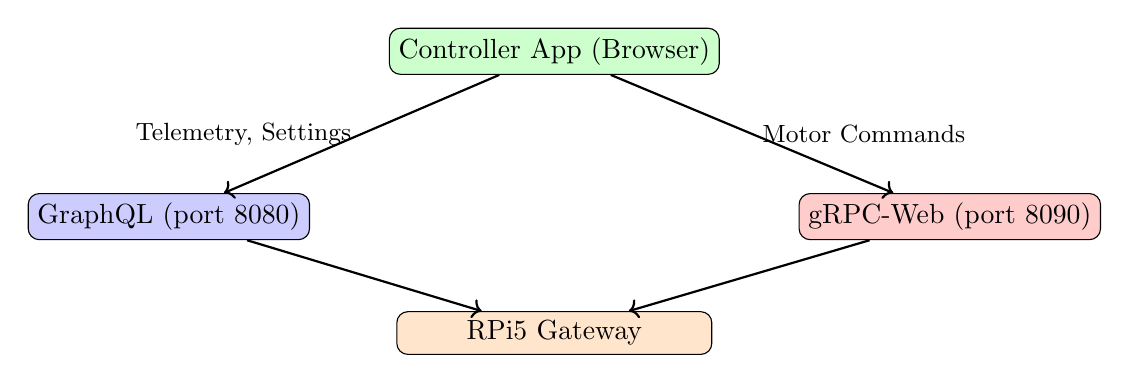
\begin{tikzpicture}[node distance=2cm, auto]
    \node[draw, rectangle, rounded corners, fill=green!20, minimum width=3cm] (browser) {Controller App (Browser)};

    \node[draw, rectangle, rounded corners, fill=blue!20, minimum width=3cm, below left=1.5cm and 1cm of browser] (graphql) {GraphQL (port 8080)};
    \node[draw, rectangle, rounded corners, fill=red!20, minimum width=3cm, below right=1.5cm and 1cm of browser] (grpc) {gRPC-Web (port 8090)};

    \node[draw, rectangle, rounded corners, fill=orange!20, minimum width=4cm, below=3cm of browser] (gateway) {RPi5 Gateway};

    \draw[->, thick] (browser) -- (graphql) node[midway, left, font=\small] {Telemetry, Settings};
    \draw[->, thick] (browser) -- (grpc) node[midway, right, font=\small] {Motor Commands};
    \draw[->, thick] (graphql) -- (gateway);
    \draw[->, thick] (grpc) -- (gateway);
\end{tikzpicture}
\caption{gRPC + GraphQL Hybrid Architecture}
\end{figure}

\textbf{Advantages:}
\begin{itemize}
    \item gRPC binary format provides fastest motor command transmission
    \item GraphQL enables flexible queries for complex UI data needs
    \item Clear separation of concerns: real-time control vs. data queries
    \item Both protocols are industry standards with excellent tooling
\end{itemize}

\textbf{Disadvantages:}
\begin{itemize}
    \item Two different APIs to maintain
    \item gRPC-Web requires Envoy proxy as translator
    \item More complex client code (two client libraries)
\end{itemize}

\subsubsection{Why This Was Selected for STAR}

\begin{enumerate}
    \item \textbf{Low-Latency Motor Control}: gRPC's binary Protobuf format minimizes serialization overhead for time-critical motor commands.

    \item \textbf{Flexible Telemetry Queries}: GraphQL subscriptions provide real-time telemetry streaming with selective field fetching.

    \item \textbf{Offline Capability}: Apollo Client (GraphQL) has excellent caching and offline support built-in.

    \item \textbf{Latency Acceptability}: For motor commands, even 10-30ms latency from browser to RPi5 is acceptable because:
    \begin{itemize}
        \item The ESP32 maintains autonomous 1kHz PID control between commands
        \item Human reaction time is approximately 200-300ms
        \item The critical real-time path is RPi5 $\rightarrow$ ESP32 (SPI), not Controller $\rightarrow$ RPi5
    \end{itemize}
\end{enumerate}

\subsection{Packet Format Comparison}

\subsubsection{Protobuf (gRPC) Binary Encoding}

Protobuf uses a compact binary format that excludes field names:

\begin{lstlisting}[language=Protobuf, caption=Protobuf Message Definition]
message VelocityCommand {
    float left_velocity = 1;   // 4 bytes + tag
    float right_velocity = 2;  // 4 bytes + tag
    uint64 timestamp = 3;      // 1-10 bytes (varint)
}
\end{lstlisting}

\textbf{Wire format example} (VelocityCommand with left=1.0, right=0.5, timestamp=1702500000000):
\begin{verbatim}
0D 00 00 80 3F  // field 1 (float): 1.0
15 00 00 00 3F  // field 2 (float): 0.5
18 80 A0 CF EE E5 31  // field 3 (varint): timestamp
\end{verbatim}

\textbf{Total size: approximately 17 bytes}

\subsubsection{JSON (GraphQL) Text Encoding}

Equivalent JSON payload:
\begin{lstlisting}[language=json, caption=JSON Equivalent]
{
  "leftVelocity": 1.0,
  "rightVelocity": 0.5,
  "timestamp": 1702500000000
}
\end{lstlisting}

\textbf{Total size: approximately 65 bytes} (3.8x larger)

\subsubsection{Serialization Performance}

Based on industry benchmarks\footnote{Source: Ambassador Labs, Protobuf vs JSON Performance Analysis, 2024}:

\begin{table}[H]
\centering
\begin{tabular}{|l|c|c|c|}
\hline
\textbf{Metric} & \textbf{Protobuf} & \textbf{JSON} & \textbf{Difference} \\
\hline
Message Size & 17 bytes & 65 bytes & 3.8x smaller \\
Serialization (JVM) & 1.2 $\mu$s & 4.5 $\mu$s & 3.75x faster \\
Deserialization (JVM) & 0.8 $\mu$s & 3.2 $\mu$s & 4x faster \\
Network Latency (1Mbps) & 0.14 ms & 0.52 ms & 3.7x faster \\
\hline
\end{tabular}
\caption{Protobuf vs JSON Performance Comparison}
\end{table}

% ============================================================================
% SECTION 3: SYSTEM ARCHITECTURE
% ============================================================================
\section{System Architecture}

\subsection{Network Topology}

\begin{figure}[H]
\centering
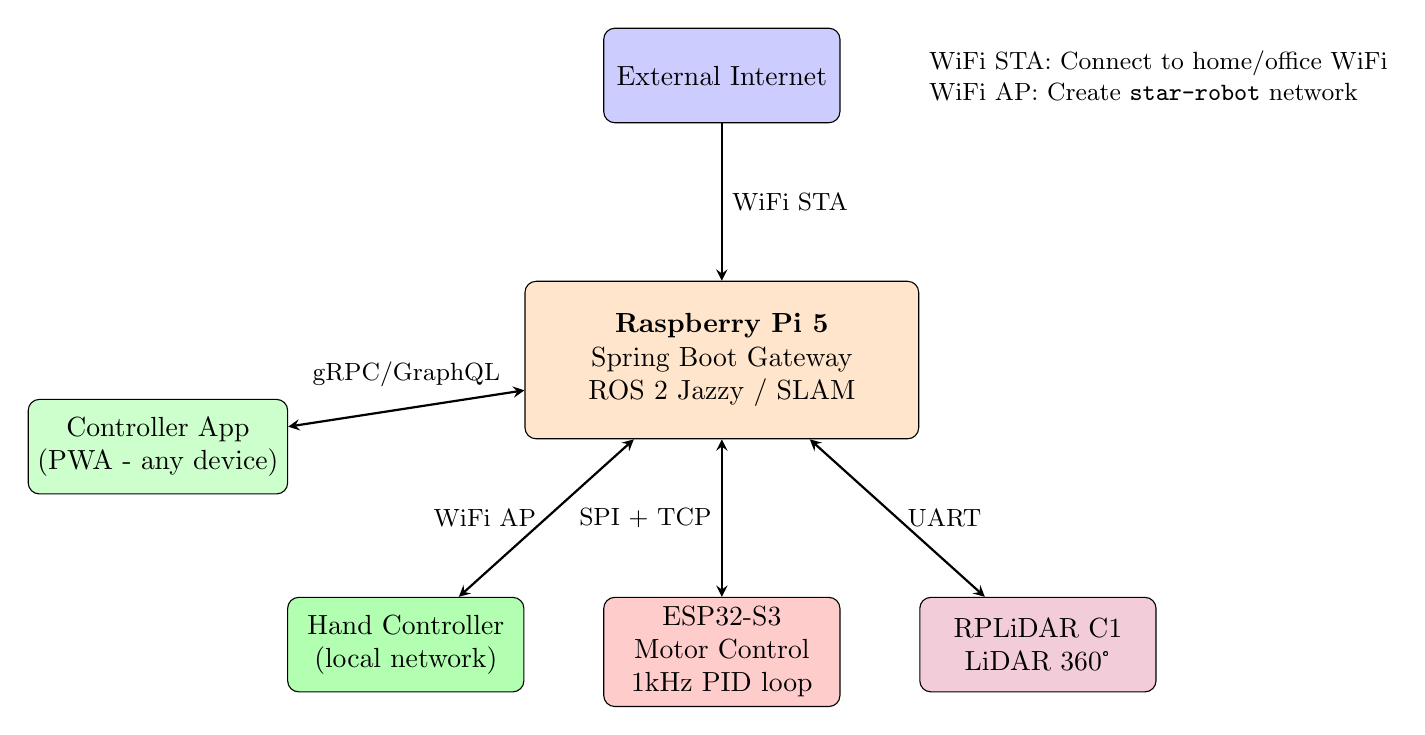
\begin{tikzpicture}[
    node distance=1.5cm,
    box/.style={draw, rectangle, rounded corners, minimum width=3cm, minimum height=1.2cm, align=center},
    arrow/.style={->, thick, >=stealth}
]
    % External Internet
    \node[box, fill=blue!20] (internet) {External Internet};

    % WiFi modes explanation
    \node[right=1cm of internet, font=\small, align=left] (wifi_note) {
        WiFi STA: Connect to home/office WiFi\\
        WiFi AP: Create \texttt{star-robot} network
    };

    % Controller App
    \node[box, fill=green!20, below left=3.5cm and 4cm of internet] (controller) {Controller App\\(PWA - any device)};

    % RPi5
    \node[box, fill=orange!20, minimum width=5cm, minimum height=2cm, below=2cm of internet] (rpi) {
        \textbf{Raspberry Pi 5}\\
        Spring Boot Gateway\\
        ROS 2 Jazzy / SLAM
    };

    % Hand Controller
    \node[box, fill=green!30, below left=2cm and 0cm of rpi] (hand) {Hand Controller\\(local network)};

    % ESP32
    \node[box, fill=red!20, below=2cm of rpi] (esp32) {ESP32-S3\\Motor Control\\1kHz PID loop};

    % LiDAR
    \node[box, fill=purple!20, below right=2cm and 0cm of rpi] (lidar) {RPLiDAR C1\\LiDAR 360\textdegree};

    % Connections
    \draw[arrow] (internet) -- node[right, font=\small] {WiFi STA} (rpi);
    \draw[arrow, <->] (controller) -- node[above, font=\small, yshift=0.15cm] {gRPC/GraphQL} (rpi);
    \draw[arrow, <->] (hand) -- node[left, font=\small] {WiFi AP} (rpi);
    \draw[arrow, <->] (rpi) -- node[left, font=\small] {SPI + TCP} (esp32);
    \draw[arrow, <->] (rpi) -- node[right, font=\small] {UART} (lidar);

\end{tikzpicture}
\caption{Complete Network Topology}
\end{figure}

\subsection{Dual WiFi Mode Operation}

The Raspberry Pi 5 operates in \textbf{simultaneous dual WiFi mode}:

\begin{enumerate}
    \item \textbf{Station (STA) Mode}: Connects to external internet for remote access
    \begin{itemize}
        \item Enables control from anywhere with internet access
        \item Allows firmware updates and remote debugging
    \end{itemize}

    \item \textbf{Access Point (AP) Mode}: Creates local \texttt{star-robot} network
    \begin{itemize}
        \item Provides low-latency local control
        \item ESP32 connects to this network for TCP fallback
        \item Hand controller connects for direct operation
    \end{itemize}
\end{enumerate}

\subsection{Software Stack Overview}

\begin{figure}[H]
\centering
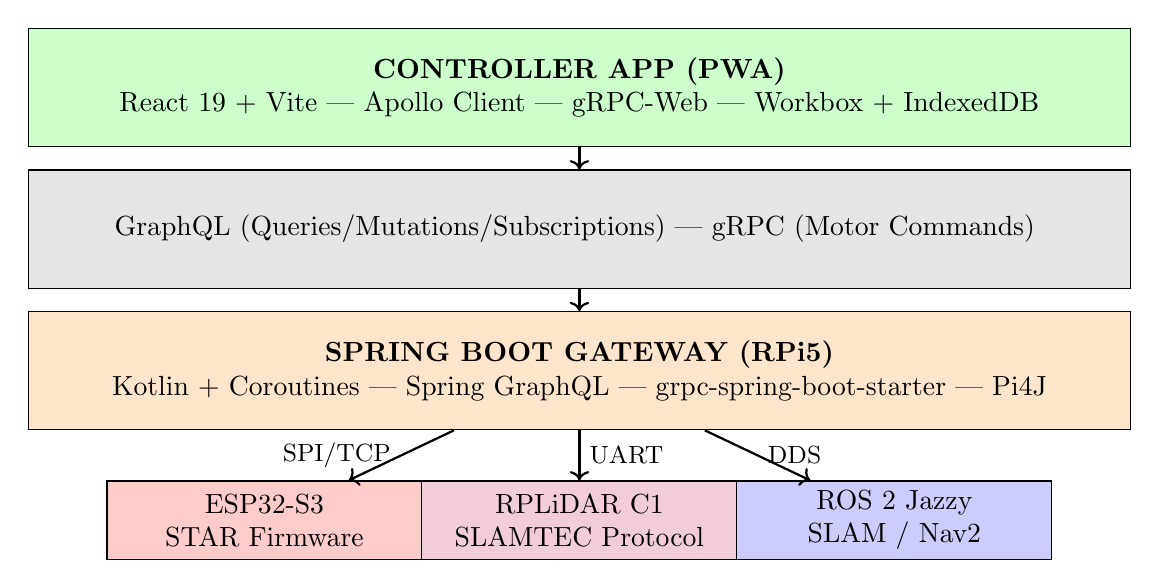
\begin{tikzpicture}[
    layer/.style={draw, rectangle, minimum width=14cm, minimum height=1.5cm, align=center},
    sublayer/.style={draw, rectangle, minimum width=4cm, minimum height=1cm, align=center}
]
    % Controller App Layer
    \node[layer, fill=green!20] (frontend) at (0,6) {
        \textbf{CONTROLLER APP (PWA)}\\
        React 19 + Vite | Apollo Client | gRPC-Web | Workbox + IndexedDB
    };

    % Protocol Layer
    \node[layer, fill=gray!20] (protocol) at (0,4.2) {
        GraphQL (Queries/Mutations/Subscriptions) | gRPC (Motor Commands)
    };

    % Gateway Layer
    \node[layer, fill=orange!20] (gateway) at (0,2.4) {
        \textbf{SPRING BOOT GATEWAY (RPi5)}\\
        Kotlin + Coroutines | Spring GraphQL | grpc-spring-boot-starter | Pi4J
    };

    % Hardware Layer
    \node[sublayer, fill=red!20] (esp32) at (-4,0.5) {ESP32-S3\\STAR Firmware};
    \node[sublayer, fill=purple!20] (lidar) at (0,0.5) {RPLiDAR C1\\SLAMTEC Protocol};
    \node[sublayer, fill=blue!20] (ros) at (4,0.5) {ROS 2 Jazzy\\SLAM / Nav2};

    % Connections
    \draw[->, thick] (frontend) -- (protocol);
    \draw[->, thick] (protocol) -- (gateway);
    \draw[->, thick] (gateway) -- node[left, font=\small] {SPI/TCP} (esp32);
    \draw[->, thick] (gateway) -- node[right, font=\small] {UART} (lidar);
    \draw[->, thick] (gateway) -- node[right, font=\small] {DDS} (ros);

\end{tikzpicture}
\caption{Software Stack Architecture}
\end{figure}

% ============================================================================
% SECTION 4: SLAM ALGORITHM SELECTION
% ============================================================================
\section{SLAM Algorithm Selection}

The STAR robot uses 2D SLAM (Simultaneous Localization and Mapping) for indoor navigation. This section documents the algorithm selection process and rationale.

\subsection{Algorithm Comparison}

Four SLAM algorithms were evaluated for the STAR platform:

\begin{table}[H]
\centering
\caption{SLAM Algorithm Comparison Matrix}
\begin{tabular}{|l|c|c|c|c|}
\hline
\textbf{Criterion (Weight)} & \textbf{SLAM Toolbox} & \textbf{Cartographer} & \textbf{Hector SLAM} & \textbf{GMapping} \\
\hline
Compute Efficiency (0.25) & 5 & 3 & 4 & 4 \\
\hline
Loop Closure Quality (0.20) & 4 & 5 & 2 & 3 \\
\hline
Indoor Accuracy (0.25) & 5 & 4 & 4 & 4 \\
\hline
ROS 2 Support (0.15) & 5 & 4 & 3 & 4 \\
\hline
Memory Usage (0.15) & 4 & 3 & 5 & 4 \\
\hline
\textbf{Weighted Score} & \textbf{4.55} & \textbf{3.75} & \textbf{3.55} & \textbf{3.80} \\
\hline
\end{tabular}
\end{table}

\textit{Scoring: 1 = Poor, 2 = Below Average, 3 = Average, 4 = Good, 5 = Excellent}

\subsection{Selection: SLAM Toolbox}

\textbf{SLAM Toolbox} was selected as the primary SLAM algorithm based on:

\begin{enumerate}
    \item \textbf{Compute Efficiency} -- Optimized for resource-constrained platforms like RPi5. Achieves 10+ Hz map updates with 360-degree LiDAR scans.

    \item \textbf{Indoor Accuracy} -- Sub-centimeter accuracy in structured indoor environments. Excellent performance with the RPLiDAR C1's 0.72-degree angular resolution.

    \item \textbf{Native ROS 2 Support} -- First-class ROS 2 Humble/Jazzy support. Developed specifically for Nav2 integration.

    \item \textbf{Flexible Operation Modes}:
    \begin{itemize}
        \item \texttt{mapping} -- Create new maps (online SLAM)
        \item \texttt{localization} -- Localize in existing maps (AMCL-like)
        \item \texttt{lifelong} -- Continuous mapping with map updates
    \end{itemize}

    \item \textbf{Serialization} -- Maps can be saved/loaded in multiple formats (PGM, YAML, binary).
\end{enumerate}

\subsection{SLAM Toolbox Configuration}

\begin{lstlisting}[language=yaml, caption=slam\_toolbox\_params.yaml]
slam_toolbox:
  ros__parameters:
    # Solver parameters
    solver_plugin: solver_plugins::CeresSolver
    ceres_linear_solver: SPARSE_NORMAL_CHOLESKY
    ceres_preconditioner: SCHUR_JACOBI
    ceres_trust_strategy: LEVENBERG_MARQUARDT
    ceres_dogleg_type: TRADITIONAL_DOGLEG
    ceres_loss_function: None

    # Frame IDs
    odom_frame: odom
    map_frame: map
    base_frame: base_link
    scan_topic: /scan
    use_scan_matching: true
    use_scan_barycenter: true

    # Resolution and range
    resolution: 0.05          # 5cm per cell (matches Nav2 costmap)
    max_laser_range: 12.0     # RPLiDAR C1 max range
    minimum_travel_distance: 0.3
    minimum_travel_heading: 0.3

    # Loop closure
    do_loop_closing: true
    loop_search_maximum_distance: 3.0
    loop_match_minimum_chain_size: 3
    loop_match_maximum_variance_coarse: 3.0
    loop_match_minimum_response_coarse: 0.35
    loop_match_minimum_response_fine: 0.45

    # Performance tuning for RPi5
    transform_publish_period: 0.05  # 20 Hz TF publish rate
    map_update_interval: 0.5        # 2 Hz map updates (reduce CPU)
    throttle_scans: 1               # Process every scan
\end{lstlisting}

\subsection{Why Not Other Algorithms?}

\begin{description}
    \item[Cartographer] Excellent loop closure but computationally expensive. Requires Lua configuration which adds complexity. Better suited for high-end compute platforms.

    \item[Hector SLAM] Fast and lightweight but lacks loop closure entirely. Drift accumulates over time in longer sessions. Best for short-duration mapping only.

    \item[GMapping] Particle filter approach with good accuracy but higher memory usage due to particle storage. ROS 2 port is community-maintained, not official.
\end{description}

\subsection{Nav2 DWA Controller Parameters}

The Dynamic Window Approach (DWA) local planner requires careful tuning for the STAR robot's physical characteristics:

\begin{table}[H]
\centering
\caption{DWA Controller Parameters}
\begin{tabular}{|l|c|l|}
\hline
\textbf{Parameter} & \textbf{Value} & \textbf{Description} \\
\hline
\multicolumn{3}{|c|}{\textbf{Velocity Limits}} \\
\hline
max\_vel\_x & 0.5 m/s & Maximum forward velocity \\
\hline
min\_vel\_x & -0.3 m/s & Maximum reverse velocity \\
\hline
max\_vel\_theta & 1.0 rad/s & Maximum angular velocity \\
\hline
min\_speed\_xy & 0.0 m/s & Minimum translational speed \\
\hline
\multicolumn{3}{|c|}{\textbf{Acceleration Limits}} \\
\hline
acc\_lim\_x & 1.0 m/s\textsuperscript{2} & Linear acceleration limit \\
\hline
acc\_lim\_theta & 2.0 rad/s\textsuperscript{2} & Angular acceleration limit \\
\hline
decel\_lim\_x & -1.5 m/s\textsuperscript{2} & Linear deceleration limit \\
\hline
decel\_lim\_theta & -2.5 rad/s\textsuperscript{2} & Angular deceleration limit \\
\hline
\multicolumn{3}{|c|}{\textbf{Trajectory Scoring}} \\
\hline
path\_distance\_bias & 32.0 & Weight for staying on global path \\
\hline
goal\_distance\_bias & 24.0 & Weight for approaching goal \\
\hline
occdist\_scale & 0.01 & Weight for avoiding obstacles \\
\hline
\multicolumn{3}{|c|}{\textbf{Costmap}} \\
\hline
inflation\_radius & 0.3 m & Obstacle inflation radius \\
\hline
cost\_scaling\_factor & 3.0 & Exponential decay rate \\
\hline
\end{tabular}
\end{table}

\begin{lstlisting}[language=yaml, caption=nav2\_params.yaml (DWA section)]
controller_server:
  ros__parameters:
    controller_frequency: 20.0  # Hz
    FollowPath:
      plugin: "dwb_core::DWBLocalPlanner"
      # Velocity limits
      max_vel_x: 0.5
      min_vel_x: -0.3
      max_vel_y: 0.0       # Differential drive - no lateral motion
      min_vel_y: 0.0
      max_vel_theta: 1.0
      min_speed_xy: 0.0
      max_speed_xy: 0.5
      min_speed_theta: 0.0
      # Acceleration limits
      acc_lim_x: 1.0
      acc_lim_y: 0.0
      acc_lim_theta: 2.0
      decel_lim_x: -1.5
      decel_lim_y: 0.0
      decel_lim_theta: -2.5
      # Trajectory generation
      vx_samples: 20
      vy_samples: 1          # Differential drive
      vtheta_samples: 40
      sim_time: 1.5          # Trajectory simulation time
      # Critics (trajectory scoring)
      critics: ["RotateToGoal", "Oscillation", "BaseObstacle",
                "GoalAlign", "PathAlign", "PathDist", "GoalDist"]
      PathAlign.scale: 32.0
      GoalAlign.scale: 24.0
      PathDist.scale: 32.0
      GoalDist.scale: 24.0
      BaseObstacle.scale: 0.01
\end{lstlisting}

% ============================================================================
% SECTION 5: ML INFERENCE PIPELINE
% ============================================================================
\section{ML Inference Pipeline}

The STAR robot uses machine learning for person detection as part of its safety system. This section documents the model selection and inference pipeline.

\subsection{Model Selection}

\begin{table}[H]
\centering
\caption{Person Detection Model Comparison}
\begin{tabular}{|l|c|c|c|c|}
\hline
\textbf{Model} & \textbf{Size (MB)} & \textbf{mAP@0.5} & \textbf{RPi5 FPS} & \textbf{Quantization} \\
\hline
YOLOv8n INT8 & 3.2 & 0.37 & 15-18 & INT8 \\
\hline
YOLOv5n FP16 & 7.5 & 0.35 & 8-10 & FP16 \\
\hline
MobileNet-SSD & 4.8 & 0.31 & 12-15 & INT8 \\
\hline
EfficientDet-Lite0 & 4.4 & 0.33 & 10-12 & INT8 \\
\hline
\end{tabular}
\end{table}

\textbf{YOLOv8n INT8} was selected for its optimal balance of accuracy and performance on the Raspberry Pi 5.

\subsection{Model Architecture}

\begin{itemize}
    \item \textbf{Base Model}: YOLOv8n (nano variant)
    \item \textbf{Input Resolution}: 320x320 (reduced from 640x640 for speed)
    \item \textbf{Quantization}: INT8 post-training quantization via TensorFlow Lite
    \item \textbf{Classes}: Single class (person) for focused detection
    \item \textbf{Inference Backend}: TensorFlow Lite with XNNPACK delegate
\end{itemize}

\subsection{Inference Pipeline}

\begin{lstlisting}[language=Python, caption=person\_detector.py]
import cv2
import numpy as np
from tflite_runtime.interpreter import Interpreter

class PersonDetector:
    def __init__(self, model_path: str = "yolov8n_int8.tflite"):
        # Load TFLite model with XNNPACK delegate for ARM optimization
        self.interpreter = Interpreter(
            model_path=model_path,
            num_threads=4  # Use all 4 Cortex-A76 cores
        )
        self.interpreter.allocate_tensors()

        self.input_details = self.interpreter.get_input_details()
        self.output_details = self.interpreter.get_output_details()
        self.input_shape = self.input_details[0]['shape'][1:3]  # (320, 320)

        # Detection thresholds
        self.confidence_threshold = 0.5
        self.nms_threshold = 0.4

    def preprocess(self, frame: np.ndarray) -> np.ndarray:
        """Resize and normalize input frame."""
        resized = cv2.resize(frame, tuple(self.input_shape))
        # INT8 quantization: scale to 0-255 range
        normalized = resized.astype(np.uint8)
        return np.expand_dims(normalized, axis=0)

    def detect(self, frame: np.ndarray) -> list:
        """Run inference and return person detections."""
        input_data = self.preprocess(frame)
        self.interpreter.set_tensor(
            self.input_details[0]['index'],
            input_data
        )
        self.interpreter.invoke()

        # Parse YOLO output format
        output = self.interpreter.get_tensor(
            self.output_details[0]['index']
        )
        detections = self._parse_output(output, frame.shape)
        return detections

    def _parse_output(self, output: np.ndarray,
                      original_shape: tuple) -> list:
        """Convert YOLO output to bounding boxes."""
        detections = []
        h, w = original_shape[:2]
        scale_x, scale_y = w / self.input_shape[1], h / self.input_shape[0]

        for detection in output[0]:
            confidence = detection[4]
            if confidence < self.confidence_threshold:
                continue

            # Extract bounding box (center format to corner format)
            cx, cy, bw, bh = detection[:4]
            x1 = int((cx - bw / 2) * scale_x)
            y1 = int((cy - bh / 2) * scale_y)
            x2 = int((cx + bw / 2) * scale_x)
            y2 = int((cy + bh / 2) * scale_y)

            detections.append({
                'bbox': (x1, y1, x2, y2),
                'confidence': float(confidence),
                'class': 'person'
            })

        # Apply non-maximum suppression
        return self._nms(detections)

    def _nms(self, detections: list) -> list:
        """Non-maximum suppression to remove overlapping boxes."""
        if not detections:
            return []

        boxes = np.array([d['bbox'] for d in detections])
        scores = np.array([d['confidence'] for d in detections])

        indices = cv2.dnn.NMSBoxes(
            boxes.tolist(),
            scores.tolist(),
            self.confidence_threshold,
            self.nms_threshold
        )

        return [detections[i] for i in indices.flatten()]
\end{lstlisting}

\subsection{Performance Optimization}

\begin{enumerate}
    \item \textbf{XNNPACK Delegate} -- ARM-optimized SIMD operations for 2-3x speedup over default TFLite.

    \item \textbf{Multi-threading} -- Utilize all 4 Cortex-A76 cores via \texttt{num\_threads=4}.

    \item \textbf{Reduced Resolution} -- 320x320 input (vs 640x640) reduces computation by 4x with minimal accuracy loss for person detection.

    \item \textbf{Frame Skipping} -- Process every 2nd frame (15 FPS effective) to maintain system responsiveness.

    \item \textbf{ROI Processing} -- In localization mode, only process regions where persons were previously detected.
\end{enumerate}

\subsection{Integration with Safety System}

The person detector feeds into the CV Safety System (Section~\ref{sec:cv-safety}):

\begin{lstlisting}[language=Python, caption=Integration with safety pipeline]
# In main control loop
detector = PersonDetector()
camera = cv2.VideoCapture(0)

while True:
    ret, frame = camera.read()
    if not ret:
        continue

    detections = detector.detect(frame)

    for det in detections:
        # Calculate distance from bounding box size
        # (calibrated for known person height)
        bbox_height = det['bbox'][3] - det['bbox'][1]
        estimated_distance = estimate_distance(bbox_height)

        # Trigger safety response based on distance
        if estimated_distance < EMERGENCY_STOP_DISTANCE:
            robot.emergency_stop()
        elif estimated_distance < SLOW_ZONE_DISTANCE:
            robot.reduce_speed(0.5)  # 50% max speed
\end{lstlisting}

% ============================================================================
% SECTION 6: CV SAFETY SYSTEM
% ============================================================================
\section{CV Safety System}
\label{sec:cv-safety}

The computer vision safety system provides an additional layer of protection beyond LiDAR-based obstacle detection. It uses the USB camera and YOLOv8n person detector to identify humans and adjust robot behavior accordingly.

\subsection{Safety Zones}

\begin{figure}[H]
\centering
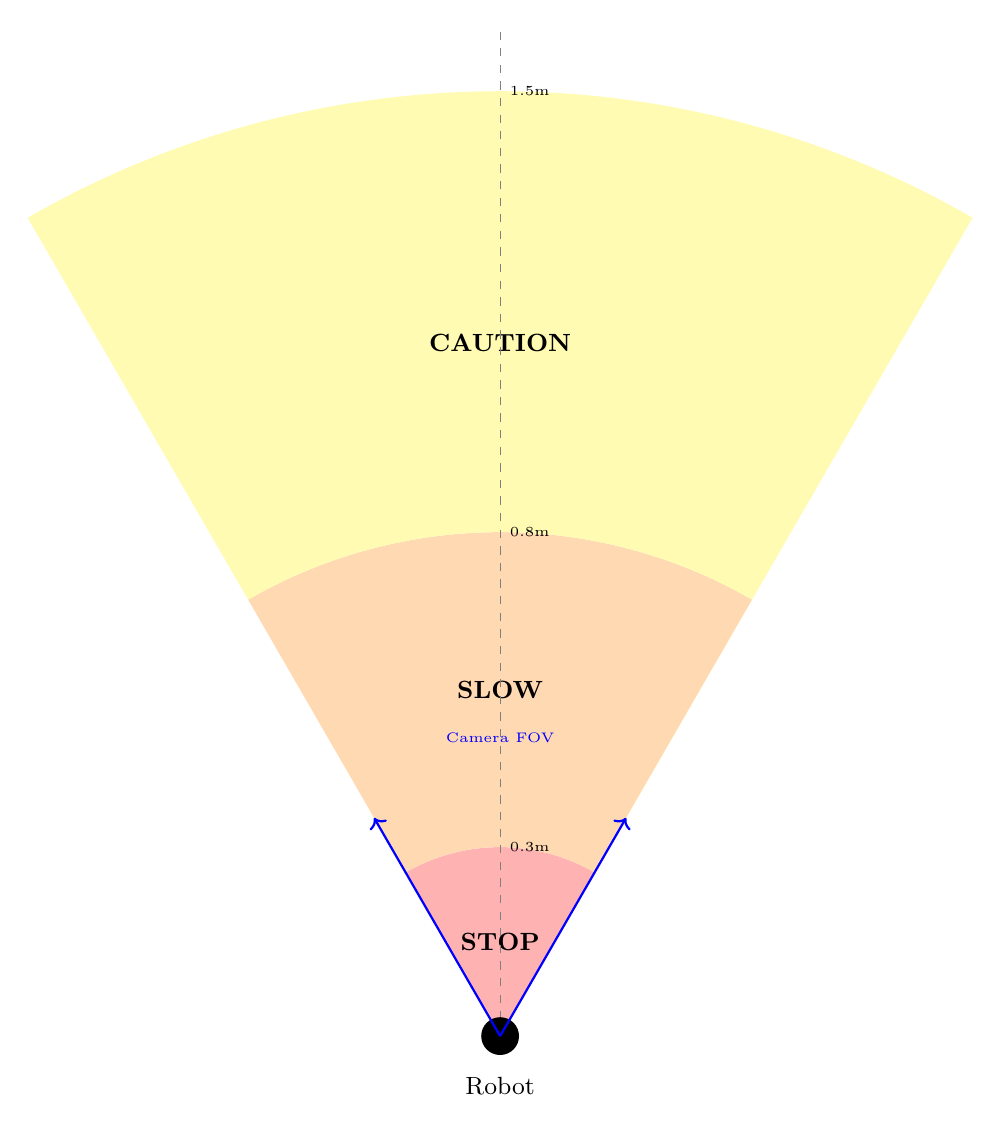
\begin{tikzpicture}[scale=0.8]
    % Draw safety zones as concentric arcs (robot FOV is forward-facing camera)
    \fill[red!30] (0,0) -- (60:3) arc (60:120:3) -- cycle;
    \fill[orange!30] (0,0) -- (60:8) arc (60:120:8) -- (120:3) arc (120:60:3) -- cycle;
    \fill[yellow!30] (0,0) -- (60:15) arc (60:120:15) -- (120:8) arc (120:60:8) -- cycle;

    % Labels for zones
    \node[font=\small\bfseries] at (90:1.5) {STOP};
    \node[font=\small\bfseries] at (90:5.5) {SLOW};
    \node[font=\small\bfseries] at (90:11) {CAUTION};

    % Distance markers
    \draw[dashed, gray] (0,0) -- (90:16);
    \node[right, font=\tiny] at (90:3) {0.3m};
    \node[right, font=\tiny] at (90:8) {0.8m};
    \node[right, font=\tiny] at (90:15) {1.5m};

    % Robot representation
    \fill[black] (0,0) circle (0.3);
    \node[below, font=\small] at (0,-0.5) {Robot};

    % Camera FOV indicator
    \draw[blue, thick, ->] (0,0) -- (60:4);
    \draw[blue, thick, ->] (0,0) -- (120:4);
    \node[blue, font=\tiny, above] at (90:4.5) {Camera FOV};

\end{tikzpicture}
\caption{Safety Zone Distances (Top-Down View)}
\end{figure}

\begin{table}[H]
\centering
\caption{Safety Zone Thresholds and Responses}
\begin{tabular}{|l|c|l|}
\hline
\textbf{Zone} & \textbf{Distance} & \textbf{Robot Response} \\
\hline
Emergency Stop (Red) & $<$ 0.3 m & Immediate stop, hold position \\
\hline
Slow Zone (Orange) & 0.3 -- 0.8 m & Reduce speed to 50\% of max \\
\hline
Caution Zone (Yellow) & 0.8 -- 1.5 m & Continue at current speed, log warning \\
\hline
Clear (Green) & $>$ 1.5 m & Normal operation \\
\hline
\end{tabular}
\end{table}

\subsection{Distance Estimation}

Since the USB camera provides 2D images without depth information, person distance is estimated using the detected bounding box height and a calibrated person height model:

\begin{lstlisting}[language=Python, caption=Distance estimation from bounding box]
# Calibration constants (adjust based on camera focal length and mounting)
FOCAL_LENGTH_PIXELS = 600  # Camera focal length in pixels
AVERAGE_PERSON_HEIGHT_M = 1.7  # Average adult height in meters
CAMERA_HEIGHT_M = 0.3  # Robot camera mounting height

def estimate_distance(bbox_height_pixels: int,
                      frame_height: int) -> float:
    """
    Estimate distance to person using pinhole camera model.

    distance = (real_height * focal_length) / image_height

    Args:
        bbox_height_pixels: Height of person bounding box in pixels
        frame_height: Total frame height in pixels

    Returns:
        Estimated distance in meters
    """
    if bbox_height_pixels <= 0:
        return float('inf')

    # Pinhole camera model
    distance = (AVERAGE_PERSON_HEIGHT_M * FOCAL_LENGTH_PIXELS) / bbox_height_pixels

    # Apply height correction (camera is not at ground level)
    # This is a simplification; more accurate models use full pose estimation
    distance = max(0.1, distance)

    return distance

# Calibration procedure:
# 1. Place person at known distance (e.g., 1.0m, 2.0m, 3.0m)
# 2. Record bounding box heights
# 3. Calculate FOCAL_LENGTH_PIXELS = (bbox_height * distance) / person_height
# 4. Average across multiple measurements
\end{lstlisting}

\subsection{Safety State Machine}

\begin{figure}[H]
\centering
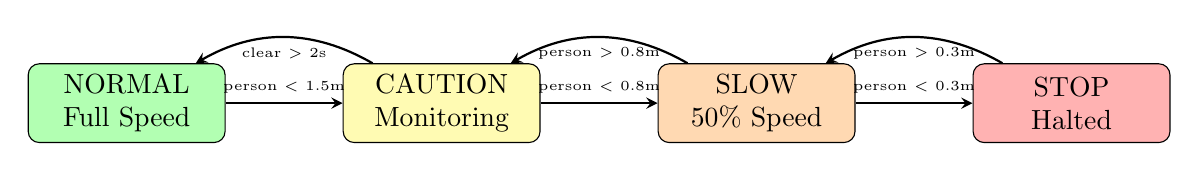
\begin{tikzpicture}[
    state/.style={draw, rectangle, rounded corners, minimum width=2.5cm, minimum height=1cm, align=center},
    arrow/.style={->, thick, >=stealth}
]
    % States
    \node[state, fill=green!30] (normal) at (0,0) {NORMAL\\Full Speed};
    \node[state, fill=yellow!30] (caution) at (4,0) {CAUTION\\Monitoring};
    \node[state, fill=orange!30] (slow) at (8,0) {SLOW\\50\% Speed};
    \node[state, fill=red!30] (stop) at (12,0) {STOP\\Halted};

    % Transitions
    \draw[arrow] (normal) -- node[above, font=\tiny] {person $<$ 1.5m} (caution);
    \draw[arrow] (caution) -- node[above, font=\tiny] {person $<$ 0.8m} (slow);
    \draw[arrow] (slow) -- node[above, font=\tiny] {person $<$ 0.3m} (stop);

    \draw[arrow, bend right=30] (caution) to node[below, font=\tiny] {clear $>$ 2s} (normal);
    \draw[arrow, bend right=30] (slow) to node[below, font=\tiny] {person $>$ 0.8m} (caution);
    \draw[arrow, bend right=30] (stop) to node[below, font=\tiny] {person $>$ 0.3m} (slow);

\end{tikzpicture}
\caption{CV Safety State Machine}
\end{figure}

\subsection{Integration with Navigation}

The CV safety system overrides navigation commands when necessary:

\begin{lstlisting}[language=Python, caption=SafetyController class]
from enum import Enum
from dataclasses import dataclass
from typing import Optional
import time

class SafetyState(Enum):
    NORMAL = "normal"
    CAUTION = "caution"
    SLOW = "slow"
    STOP = "stop"

@dataclass
class SafetyZones:
    EMERGENCY_STOP: float = 0.3   # meters
    SLOW_ZONE: float = 0.8        # meters
    CAUTION_ZONE: float = 1.5     # meters
    CLEAR_TIMEOUT: float = 2.0    # seconds before returning to normal

class SafetyController:
    def __init__(self):
        self.state = SafetyState.NORMAL
        self.last_detection_time: Optional[float] = None
        self.speed_multiplier = 1.0

    def update(self, person_distance: Optional[float]) -> SafetyState:
        """Update safety state based on nearest person distance."""
        current_time = time.time()

        if person_distance is None:
            # No person detected
            if self.last_detection_time is not None:
                elapsed = current_time - self.last_detection_time
                if elapsed > SafetyZones.CLEAR_TIMEOUT:
                    self._transition_to(SafetyState.NORMAL)
            return self.state

        self.last_detection_time = current_time

        # Determine appropriate state based on distance
        if person_distance < SafetyZones.EMERGENCY_STOP:
            self._transition_to(SafetyState.STOP)
        elif person_distance < SafetyZones.SLOW_ZONE:
            self._transition_to(SafetyState.SLOW)
        elif person_distance < SafetyZones.CAUTION_ZONE:
            self._transition_to(SafetyState.CAUTION)

        return self.state

    def _transition_to(self, new_state: SafetyState):
        if new_state != self.state:
            print(f"Safety state: {self.state.value} -> {new_state.value}")
            self.state = new_state
            self._update_speed_multiplier()

    def _update_speed_multiplier(self):
        multipliers = {
            SafetyState.NORMAL: 1.0,
            SafetyState.CAUTION: 1.0,
            SafetyState.SLOW: 0.5,
            SafetyState.STOP: 0.0,
        }
        self.speed_multiplier = multipliers[self.state]

    def apply_to_velocity(self, cmd_vel: tuple) -> tuple:
        """Apply safety multiplier to velocity command."""
        linear, angular = cmd_vel
        return (linear * self.speed_multiplier,
                angular * self.speed_multiplier)
\end{lstlisting}

% ============================================================================
% SECTION 7: BATTERY MANAGEMENT
% ============================================================================
\section{Battery Management}

The STAR robot implements a multi-threshold battery management system to ensure safe operation and prevent damage from deep discharge.

\subsection{Battery State Thresholds}

\begin{figure}[H]
\centering
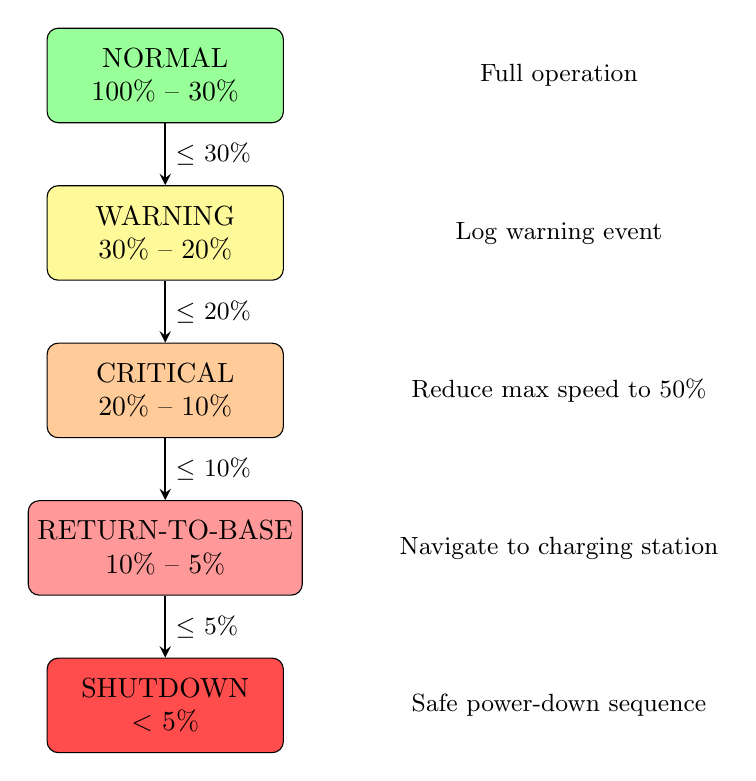
\begin{tikzpicture}[
    state/.style={draw, rectangle, rounded corners, minimum width=3cm, minimum height=1.2cm, align=center},
    arrow/.style={->, thick, >=stealth}
]
    % States arranged vertically
    \node[state, fill=green!40] (normal) at (0,6) {NORMAL\\100\% -- 30\%};
    \node[state, fill=yellow!40] (warning) at (0,4) {WARNING\\30\% -- 20\%};
    \node[state, fill=orange!40] (critical) at (0,2) {CRITICAL\\20\% -- 10\%};
    \node[state, fill=red!40] (rtb) at (0,0) {RETURN-TO-BASE\\10\% -- 5\%};
    \node[state, fill=red!70] (shutdown) at (0,-2) {SHUTDOWN\\$<$ 5\%};

    % Transitions
    \draw[arrow] (normal) -- node[right, font=\small] {$\leq$ 30\%} (warning);
    \draw[arrow] (warning) -- node[right, font=\small] {$\leq$ 20\%} (critical);
    \draw[arrow] (critical) -- node[right, font=\small] {$\leq$ 10\%} (rtb);
    \draw[arrow] (rtb) -- node[right, font=\small] {$\leq$ 5\%} (shutdown);

    % Actions on right side
    \node[align=left, font=\small] at (5,6) {Full operation};
    \node[align=left, font=\small] at (5,4) {Log warning event};
    \node[align=left, font=\small] at (5,2) {Reduce max speed to 50\%};
    \node[align=left, font=\small] at (5,0) {Navigate to charging station};
    \node[align=left, font=\small] at (5,-2) {Safe power-down sequence};

\end{tikzpicture}
\caption{Battery State Machine}
\end{figure}

\begin{table}[H]
\centering
\caption{Battery Management Thresholds}
\begin{tabular}{|c|l|l|}
\hline
\textbf{Level} & \textbf{State} & \textbf{Action} \\
\hline
100\% -- 30\% & Normal & Full operation, no restrictions \\
\hline
30\% & Warning & Log battery warning event to telemetry \\
\hline
20\% & Critical & Reduce maximum speed to 50\% \\
\hline
10\% & Return-to-Base & Abort current task, navigate to charging station \\
\hline
5\% & Emergency & Initiate safe shutdown sequence \\
\hline
\end{tabular}
\end{table}

\subsection{Battery Monitoring}

Battery voltage and state-of-charge are monitored via the ESP32's ADC with filtering:

\begin{lstlisting}[language=C, caption=Battery monitoring (ESP32)]
#include <esp_adc_cal.h>

#define BATTERY_ADC_CHANNEL     ADC1_CHANNEL_6  // GPIO34
#define BATTERY_SAMPLES         16              // Averaging samples
#define VOLTAGE_DIVIDER_RATIO   4.0             // R1=30k, R2=10k
#define BATTERY_MIN_V           10.0            // 3S LiPo empty
#define BATTERY_MAX_V           12.6            // 3S LiPo full

typedef enum {
    BATTERY_NORMAL,
    BATTERY_WARNING,
    BATTERY_CRITICAL,
    BATTERY_RTB,
    BATTERY_SHUTDOWN
} battery_state_t;

static esp_adc_cal_characteristics_t adc_chars;
static battery_state_t current_state = BATTERY_NORMAL;

void battery_init(void) {
    adc1_config_width(ADC_WIDTH_BIT_12);
    adc1_config_channel_atten(BATTERY_ADC_CHANNEL, ADC_ATTEN_DB_11);
    esp_adc_cal_characterize(ADC_UNIT_1, ADC_ATTEN_DB_11,
                             ADC_WIDTH_BIT_12, 1100, &adc_chars);
}

float battery_read_voltage(void) {
    uint32_t adc_sum = 0;

    // Multi-sample averaging for noise reduction
    for (int i = 0; i < BATTERY_SAMPLES; i++) {
        adc_sum += adc1_get_raw(BATTERY_ADC_CHANNEL);
    }
    uint32_t adc_avg = adc_sum / BATTERY_SAMPLES;

    // Convert to voltage
    uint32_t voltage_mv = esp_adc_cal_raw_to_voltage(adc_avg, &adc_chars);

    return (voltage_mv / 1000.0f) * VOLTAGE_DIVIDER_RATIO;
}

uint8_t battery_get_percentage(float voltage) {
    // Linear approximation (for LiPo, use lookup table for accuracy)
    float pct = (voltage - BATTERY_MIN_V) / (BATTERY_MAX_V - BATTERY_MIN_V);
    pct = fmaxf(0.0f, fminf(1.0f, pct));
    return (uint8_t)(pct * 100.0f);
}

battery_state_t battery_update_state(uint8_t percentage) {
    if (percentage <= 5) {
        current_state = BATTERY_SHUTDOWN;
    } else if (percentage <= 10) {
        current_state = BATTERY_RTB;
    } else if (percentage <= 20) {
        current_state = BATTERY_CRITICAL;
    } else if (percentage <= 30) {
        current_state = BATTERY_WARNING;
    } else {
        current_state = BATTERY_NORMAL;
    }
    return current_state;
}
\end{lstlisting}

\subsection{Safe Shutdown Sequence}

When battery reaches critical level (5\%), the system initiates a controlled shutdown:

\begin{enumerate}
    \item \textbf{Stop Motors} -- Immediate motor disable, engage brakes if available
    \item \textbf{Log Position} -- Save current map position to persistent storage
    \item \textbf{Notify User} -- Send critical battery notification via GraphQL subscription
    \item \textbf{Save State} -- Persist navigation state, waypoints, and settings to flash
    \item \textbf{Shutdown Sequence} -- Graceful ROS 2 node shutdown, then Linux poweroff
\end{enumerate}

% ============================================================================
% SECTION 8: REPOSITORY STRUCTURE
% ============================================================================
\section{Repository Structure}

\subsection{Directory Layout}

\begin{lstlisting}[language=bash, caption=Complete Repository Structure]
/STAR/
|-- ESP32-Firmware/           # Existing - keep as-is
|-- star-pi5-os/              # Existing - add gateway to Buildroot
|-- Schematic/                # Existing - hardware designs
|-- Locked_Inc_FTP/           # Existing - documentation
|-- docs/                     # Existing - documentation
|
|-- star-gateway/             # NEW: Spring Boot Gateway
|   |-- build.gradle.kts
|   |-- settings.gradle.kts
|   |-- src/
|   |   +-- main/
|   |       |-- kotlin/com/star/gateway/
|   |       |   |-- StarGatewayApplication.kt
|   |       |   |-- config/
|   |       |   |   |-- GraphQLConfig.kt
|   |       |   |   |-- GrpcConfig.kt
|   |       |   |   +-- CorsConfig.kt
|   |       |   |-- graphql/
|   |       |   |   |-- TelemetryController.kt
|   |       |   |   |-- SettingsController.kt
|   |       |   |   +-- NavigationController.kt
|   |       |   |-- grpc/
|   |       |   |   +-- MotorControlGrpcService.kt
|   |       |   |-- service/
|   |       |   |   |-- MotorControlService.kt
|   |       |   |   |-- TelemetryService.kt
|   |       |   |   |-- NavigationService.kt
|   |       |   |   +-- SensorFusionService.kt
|   |       |   |-- hardware/
|   |       |   |   |-- Esp32SpiAdapter.kt
|   |       |   |   |-- Esp32TcpAdapter.kt
|   |       |   |   |-- RplidarAdapter.kt
|   |       |   |   +-- Ros2Bridge.kt
|   |       |   +-- model/
|   |       |       |-- TelemetryData.kt
|   |       |       |-- MotorCommand.kt
|   |       |       +-- NavigationState.kt
|   |       |-- proto/
|   |       |   +-- motor_control.proto
|   |       +-- resources/
|   |           |-- application.yml
|   |           +-- graphql/
|   |               +-- schema.graphqls
|   +-- deployment/
|       |-- star-gateway.service    # Systemd unit
|       +-- avahi/
|           +-- star-robot.service  # mDNS config
|
|-- star-ui/                  # NEW: PWA (moved from UI-Demo)
|   |-- package.json
|   |-- vite.config.js
|   |-- public/
|   |   |-- manifest.json
|   |   +-- sw.js
|   |-- src/
|   |   |-- main.jsx
|   |   |-- App.jsx
|   |   |-- components/           # From UI-Demo
|   |   |-- pages/                # From UI-Demo
|   |   |-- hooks/
|   |   |   |-- useRobotConnection.js
|   |   |   |-- useTelemetry.js
|   |   |   +-- useMotorControl.js
|   |   |-- graphql/
|   |   |   |-- client.js
|   |   |   |-- queries.js
|   |   |   |-- mutations.js
|   |   |   +-- subscriptions.js
|   |   |-- grpc/
|   |   |   |-- client.js
|   |   |   +-- motor_control_pb.js
|   |   |-- service-worker/
|   |   |   |-- sw.js
|   |   |   +-- offline-cache.js
|   |   +-- storage/
|   |       +-- indexedDB.js
|   +-- workbox-config.js
|
+-- proto/                    # SHARED: Protobuf definitions
    +-- star/
        |-- motor_control.proto
        |-- telemetry.proto
        +-- navigation.proto
\end{lstlisting}

% ============================================================================
% SECTION 5: SPRING BOOT GATEWAY
% ============================================================================
\section{Spring Boot Gateway Implementation}

\subsection{Build Configuration}

\begin{lstlisting}[language=Kotlin, caption=build.gradle.kts]
plugins {
    kotlin("jvm") version "1.9.22"
    kotlin("plugin.spring") version "1.9.22"
    id("org.springframework.boot") version "3.2.4"
    id("io.spring.dependency-management") version "1.1.4"
    id("com.google.protobuf") version "0.9.4"
}

java {
    sourceCompatibility = JavaVersion.VERSION_17
}

repositories {
    mavenCentral()
}

dependencies {
    // Spring Boot Core
    implementation("org.springframework.boot:spring-boot-starter-webflux")
    implementation("org.springframework.boot:spring-boot-starter-actuator")

    // GraphQL
    implementation("org.springframework.boot:spring-boot-starter-graphql")

    // gRPC
    implementation("net.devh:grpc-spring-boot-starter:3.1.0.RELEASE")
    implementation("io.grpc:grpc-kotlin-stub:1.4.1")
    implementation("io.grpc:grpc-protobuf:1.60.1")
    implementation("com.google.protobuf:protobuf-kotlin:3.25.2")

    // Kotlin Coroutines
    implementation("org.jetbrains.kotlinx:kotlinx-coroutines-core:1.8.0")
    implementation("org.jetbrains.kotlinx:kotlinx-coroutines-reactor:1.8.0")
    implementation("io.projectreactor.kotlin:reactor-kotlin-extensions")

    // Hardware Access (Pi4J for SPI/GPIO)
    // Pi4J 2.6+ required for Raspberry Pi 5 (RP1 chip support via GpioD)
    implementation("com.pi4j:pi4j-core:2.6.1")
    implementation("com.pi4j:pi4j-plugin-raspberrypi:2.6.1")
    implementation("com.pi4j:pi4j-plugin-gpiod:2.6.1")  // Required for RPi5
    implementation("com.pi4j:pi4j-plugin-linuxfs:2.6.1")

    // Metrics
    implementation("io.micrometer:micrometer-registry-prometheus")

    // JSON Processing
    implementation("com.fasterxml.jackson.module:jackson-module-kotlin")

    // Kotlin Reflection
    implementation("org.jetbrains.kotlin:kotlin-reflect")

    // Testing
    testImplementation("org.springframework.boot:spring-boot-starter-test")
    testImplementation("io.projectreactor:reactor-test")
}

protobuf {
    protoc {
        artifact = "com.google.protobuf:protoc:3.25.2"
    }
    plugins {
        id("grpc") {
            artifact = "io.grpc:protoc-gen-grpc-java:1.60.1"
        }
        id("grpckt") {
            artifact = "io.grpc:protoc-gen-grpc-kotlin:1.4.1:jdk8@jar"
        }
    }
    generateProtoTasks {
        all().forEach {
            it.plugins {
                id("grpc")
                id("grpckt")
            }
            it.builtins {
                id("kotlin")
            }
        }
    }
}

tasks.withType<org.jetbrains.kotlin.gradle.tasks.KotlinCompile> {
    kotlinOptions {
        freeCompilerArgs += "-Xjsr305=strict"
        jvmTarget = "17"
    }
}
\end{lstlisting}

\subsection{Application Configuration}

\begin{lstlisting}[language=yaml, caption=application.yml]
spring:
  application:
    name: star-gateway
  graphql:
    graphiql:
      enabled: true
      path: /graphiql
    websocket:
      path: /graphql-ws
    schema:
      locations: classpath:graphql/
  main:
    banner-mode: off

server:
  port: 8080

grpc:
  server:
    port: 9090

# Hardware configuration
star:
  esp32:
    spi:
      enabled: true
      bus: 0
      chip-select: 0
      speed-hz: 10000000  # 10 MHz for motor control
      mode: 0
    tcp:
      enabled: true
      host: 192.168.4.2  # ESP32 IP on AP network
      port: 5000
      timeout-ms: 100
      retry-attempts: 3
  lidar:
    serial-port: /dev/ttyAMA0
    baud-rate: 460800
    protocol: SLAMTEC
    scan-rate-hz: 10

# Actuator endpoints for health checks
management:
  endpoints:
    web:
      exposure:
        include: health,prometheus,info,metrics
  endpoint:
    health:
      show-details: always
  metrics:
    tags:
      application: star-gateway

logging:
  level:
    com.star.gateway: DEBUG
    org.springframework.graphql: INFO
\end{lstlisting}

\subsection{Six-Layer Software Architecture}

The STAR system follows a strict six-layer architecture spanning from the remote UI to embedded firmware:

\begin{figure}[H]
\centering
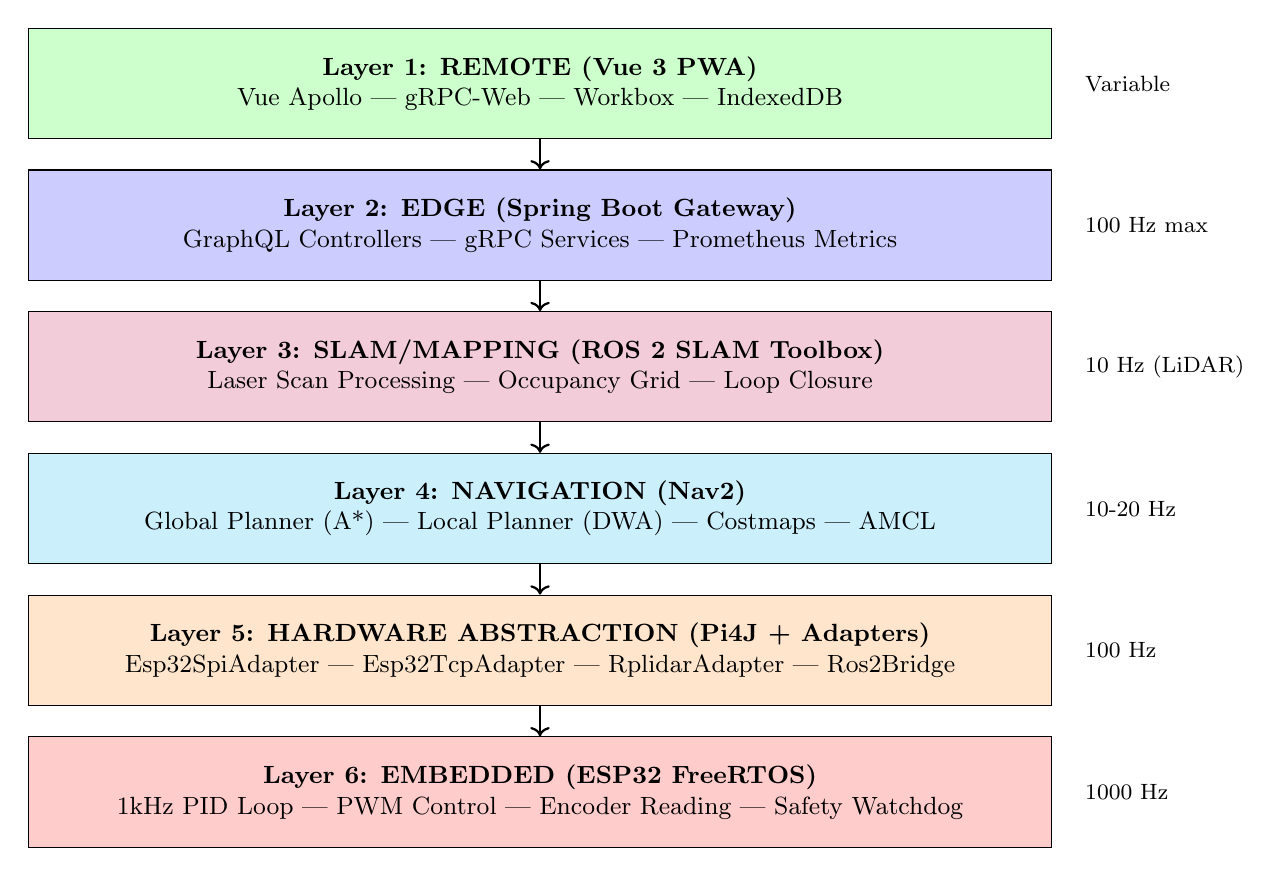
\begin{tikzpicture}[
    layer/.style={draw, rectangle, minimum width=13cm, minimum height=1.4cm, align=center, font=\small}
]
    % Layer 1: Remote
    \node[layer, fill=green!20] (remote) at (0,9) {
        \textbf{Layer 1: REMOTE (Vue 3 PWA)}\\
        Vue Apollo | gRPC-Web | Workbox | IndexedDB
    };

    % Layer 2: Edge
    \node[layer, fill=blue!20] (edge) at (0,7.2) {
        \textbf{Layer 2: EDGE (Spring Boot Gateway)}\\
        GraphQL Controllers | gRPC Services | Prometheus Metrics
    };

    % Layer 3: SLAM
    \node[layer, fill=purple!20] (slam) at (0,5.4) {
        \textbf{Layer 3: SLAM/MAPPING (ROS 2 SLAM Toolbox)}\\
        Laser Scan Processing | Occupancy Grid | Loop Closure
    };

    % Layer 4: Navigation
    \node[layer, fill=cyan!20] (nav) at (0,3.6) {
        \textbf{Layer 4: NAVIGATION (Nav2)}\\
        Global Planner (A*) | Local Planner (DWA) | Costmaps | AMCL
    };

    % Layer 5: Hardware Abstraction
    \node[layer, fill=orange!20] (hal) at (0,1.8) {
        \textbf{Layer 5: HARDWARE ABSTRACTION (Pi4J + Adapters)}\\
        Esp32SpiAdapter | Esp32TcpAdapter | RplidarAdapter | Ros2Bridge
    };

    % Layer 6: Embedded
    \node[layer, fill=red!20] (embedded) at (0,0) {
        \textbf{Layer 6: EMBEDDED (ESP32 FreeRTOS)}\\
        1kHz PID Loop | PWM Control | Encoder Reading | Safety Watchdog
    };

    % Arrows
    \draw[->, thick] (remote) -- (edge);
    \draw[->, thick] (edge) -- (slam);
    \draw[->, thick] (slam) -- (nav);
    \draw[->, thick] (nav) -- (hal);
    \draw[->, thick] (hal) -- (embedded);

    % Update rates on the right
    \node[right, font=\footnotesize] at (6.8,9) {Variable};
    \node[right, font=\footnotesize] at (6.8,7.2) {100 Hz max};
    \node[right, font=\footnotesize] at (6.8,5.4) {10 Hz (LiDAR)};
    \node[right, font=\footnotesize] at (6.8,3.6) {10-20 Hz};
    \node[right, font=\footnotesize] at (6.8,1.8) {100 Hz};
    \node[right, font=\footnotesize] at (6.8,0) {1000 Hz};

\end{tikzpicture}
\caption{Six-Layer Software Architecture with Update Frequencies}
\end{figure}

\subsubsection{Layer Responsibilities}

\begin{description}[style=nextline, leftmargin=1cm]
    \item[Layer 1 - Remote (Vue 3 PWA)] User interface running in browser or as installed PWA. Handles user input, displays telemetry, provides offline capability via service workers and IndexedDB.

    \item[Layer 2 - Edge (Spring Boot Gateway)] API gateway running on RPi5. Translates between web protocols (GraphQL/gRPC) and robot internals. Manages authentication, rate limiting, and metrics.

    \item[Layer 3 - SLAM/Mapping (ROS 2 SLAM Toolbox)] Processes LiDAR scans to build occupancy grid maps. Handles loop closure detection and map optimization. Updates at LiDAR scan rate (10 Hz).

    \item[Layer 4 - Navigation (Nav2)] Path planning and obstacle avoidance. Global planner (A*) runs at 10 Hz, local planner (DWA) runs at 20 Hz. Publishes velocity commands to Layer 5.

    \item[Layer 5 - Hardware Abstraction (Pi4J + Adapters)] Interfaces between ROS 2 and physical hardware. Communicates with ESP32 via SPI (primary) and TCP (fallback). Reads LiDAR via UART (rplidar\_ros2 driver).

    \item[Layer 6 - Embedded (ESP32 FreeRTOS)] Real-time motor control at 1 kHz. Runs PID loops, reads encoders, generates PWM signals. Maintains safe operation even if higher layers fail.
\end{description}

\subsubsection{Control Timing Hierarchy}

The STAR robot operates with a multi-rate control hierarchy, where each layer runs at a frequency appropriate to its function:

\begin{figure}[H]
\centering
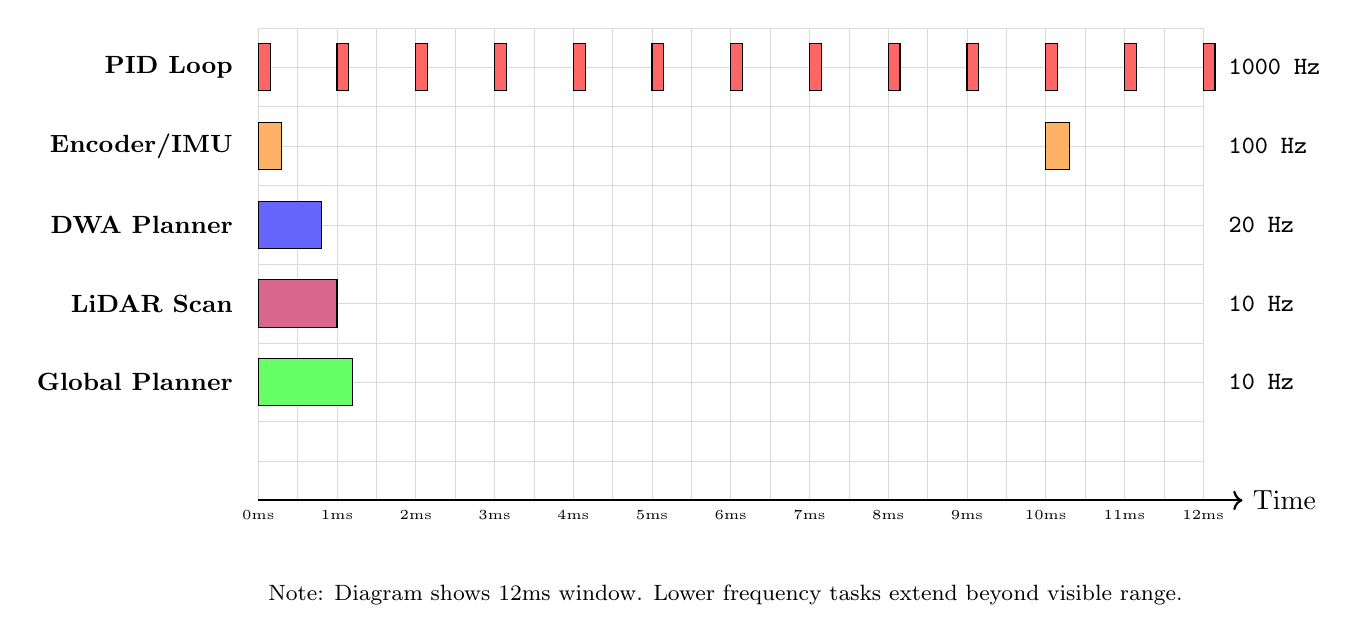
\begin{tikzpicture}[
    timebar/.style={draw, rectangle, minimum height=0.8cm, fill=#1},
    label/.style={font=\small\bfseries},
    freq/.style={font=\small\ttfamily}
]
    % Background grid showing time
    \draw[gray!30, very thin] (0,0) grid[step=0.5] (12,6);

    % Time axis
    \draw[->, thick] (0,0) -- (12.5,0) node[right] {Time};
    \foreach \x in {0,1,2,3,4,5,6,7,8,9,10,11,12} {
        \node[below, font=\tiny] at (\x,0) {\x ms};
    }

    % 1000 Hz PID Loop (ESP32) - every 1ms
    \foreach \x in {0,1,2,3,4,5,6,7,8,9,10,11,12} {
        \draw[fill=red!60] (\x,5.2) rectangle (\x+0.15,5.8);
    }
    \node[label, left] at (-0.2,5.5) {PID Loop};
    \node[freq, right] at (12.2,5.5) {1000 Hz};

    % 100 Hz Encoder/IMU (ESP32) - every 10ms
    \foreach \x in {0,10} {
        \draw[fill=orange!60] (\x,4.2) rectangle (\x+0.3,4.8);
    }
    \node[label, left] at (-0.2,4.5) {Encoder/IMU};
    \node[freq, right] at (12.2,4.5) {100 Hz};

    % 20 Hz DWA Local Planner - every 50ms (not visible in 12ms window, show one)
    \draw[fill=blue!60] (0,3.2) rectangle (0.8,3.8);
    \node[label, left] at (-0.2,3.5) {DWA Planner};
    \node[freq, right] at (12.2,3.5) {20 Hz};

    % 10 Hz LiDAR Scan - every 100ms (not visible in 12ms window, show one)
    \draw[fill=purple!60] (0,2.2) rectangle (1.0,2.8);
    \node[label, left] at (-0.2,2.5) {LiDAR Scan};
    \node[freq, right] at (12.2,2.5) {10 Hz};

    % 10 Hz Global Planner - every 100ms (not visible in 12ms window, show one)
    \draw[fill=green!60] (0,1.2) rectangle (1.2,1.8);
    \node[label, left] at (-0.2,1.5) {Global Planner};
    \node[freq, right] at (12.2,1.5) {10 Hz};

    % Legend
    \node[align=left, font=\footnotesize] at (6,-1.2) {
        Note: Diagram shows 12ms window. Lower frequency tasks extend beyond visible range.
    };

\end{tikzpicture}
\caption{Control Timing Hierarchy (12ms Window)}
\end{figure}

\begin{table}[H]
\centering
\caption{Control Loop Frequencies and Responsibilities}
\begin{tabular}{|l|c|l|l|}
\hline
\textbf{Control Loop} & \textbf{Frequency} & \textbf{Period} & \textbf{Processor} \\
\hline
PID Motor Control & 1000 Hz & 1 ms & ESP32 (FreeRTOS) \\
\hline
Encoder/IMU Sampling & 100 Hz & 10 ms & ESP32 (FreeRTOS) \\
\hline
DWA Local Planner & 20 Hz & 50 ms & RPi5 (Nav2) \\
\hline
LiDAR Scan Processing & 10 Hz & 100 ms & RPi5 (ROS 2) \\
\hline
Global Path Planner & 10 Hz & 100 ms & RPi5 (Nav2) \\
\hline
Telemetry Publishing & 10 Hz & 100 ms & RPi5 (Spring Boot) \\
\hline
Map Updates & 2 Hz & 500 ms & RPi5 (SLAM Toolbox) \\
\hline
\end{tabular}
\end{table}

\textbf{Timing Design Rationale}:
\begin{itemize}
    \item \textbf{1000 Hz PID} -- Required for smooth motor control and quick response to disturbances. FreeRTOS ensures deterministic timing.

    \item \textbf{100 Hz Sensor Sampling} -- Captures high-frequency vibrations and provides accurate velocity estimates via differentiation.

    \item \textbf{20 Hz DWA} -- Fast enough for obstacle avoidance at max velocity (0.5 m/s = 2.5cm per cycle), slow enough to not overload CPU.

    \item \textbf{10 Hz LiDAR} -- Fixed by RPLiDAR C1 hardware. Sufficient for indoor navigation at walking speeds.

    \item \textbf{10 Hz Global Planner} -- Path replanning happens infrequently; 10 Hz allows quick re-routing while minimizing CPU load.
\end{itemize}

\subsection{GraphQL Schema}

\begin{lstlisting}[language=GraphQL, caption=schema.graphqls]
# Query operations - read-only data fetching
type Query {
    telemetry: Telemetry!
    systemStatus: SystemStatus!
    settings: Settings!
    navigationState: NavigationState!
    telemetryHistory(limit: Int = 100): [TelemetrySnapshot!]!
}

# Mutation operations - state changes
type Mutation {
    setMode(mode: RobotMode!): Boolean!
    emergencyStop: Boolean!
    setSettings(input: SettingsInput!): Settings!
    addWaypoint(x: Float!, y: Float!): Waypoint!
    clearWaypoints: Boolean!
    startNavigation: Boolean!
    stopNavigation: Boolean!
}

# Subscription operations - real-time streams
type Subscription {
    telemetryStream: Telemetry!
    lidarScan: LidarScan!
    eventLog: Event!
}

# Core telemetry data structure
type Telemetry {
    imu: ImuData!
    gps: GpsData!
    battery: Float!
    wifiSignal: Int!
    cpuUsage: Float!
    temperature: Float!
    motorLoad: Float!
    timestamp: String!
}

type ImuData {
    pitch: Float!
    roll: Float!
    yaw: Float!
    velocity: Float!
    accelerationX: Float!
    accelerationY: Float!
    accelerationZ: Float!
}

type GpsData {
    latitude: Float!
    longitude: Float!
    altitude: Float!
}

type LidarScan {
    points: [LidarPoint!]!
    timestamp: String!
}

type LidarPoint {
    angle: Float!
    distance: Float!
    intensity: Float!
}

type SystemStatus {
    connectionStatus: ConnectionStatus!
    mode: RobotMode!
    esp32Connected: Boolean!
    lidarConnected: Boolean!
    rosConnected: Boolean!
}

type NavigationState {
    currentPosition: Position!
    path: [Position!]!
    waypoints: [Waypoint!]!
    isNavigating: Boolean!
}

type Position {
    x: Float!
    y: Float!
    heading: Float!
}

type Waypoint {
    id: ID!
    x: Float!
    y: Float!
    label: String
}

type Event {
    timestamp: String!
    message: String!
    type: EventType!
}

type Settings {
    maxSpeed: Float!
    safetyLockEnabled: Boolean!
    autonomousEnabled: Boolean!
    lidarEnabled: Boolean!
}

input SettingsInput {
    maxSpeed: Float
    safetyLockEnabled: Boolean
    autonomousEnabled: Boolean
    lidarEnabled: Boolean
}

enum RobotMode {
    IDLE
    MANUAL
    AUTONOMOUS
    MAPPING
    EMERGENCY_STOP
}

enum ConnectionStatus {
    CONNECTED
    DISCONNECTED
    CONNECTING
    ERROR
}

enum EventType {
    INFO
    SUCCESS
    WARNING
    ERROR
}
\end{lstlisting}

\subsection{gRPC Protobuf Definition}

\begin{lstlisting}[language=Protobuf, caption=motor\_control.proto]
syntax = "proto3";

package star.motor;

option java_package = "com.star.gateway.proto";
option java_outer_classname = "MotorControlProto";
option java_multiple_files = true;

// Motor control service for low-latency commands
service MotorControl {
    // Unary RPCs (single request-response)
    rpc SetVelocity(VelocityCommand) returns (CommandResponse);
    rpc EmergencyStop(EmptyRequest) returns (CommandResponse);
    rpc SetMotorPower(MotorPowerCommand) returns (CommandResponse);

    // Server streaming (continuous encoder feedback)
    rpc StreamEncoderData(EmptyRequest) returns (stream EncoderData);
}

// Velocity command for differential drive
message VelocityCommand {
    float left_velocity = 1;   // m/s, range: -2.0 to 2.0
    float right_velocity = 2;  // m/s, range: -2.0 to 2.0
    uint64 timestamp = 3;      // Unix timestamp in milliseconds
}

// Direct motor power control
message MotorPowerCommand {
    int32 motor_id = 1;        // Motor index: 0-3
    float power = 2;           // Power level: -1.0 to 1.0
}

// Standard command response
message CommandResponse {
    bool success = 1;          // True if command executed
    string message = 2;        // Human-readable status
    uint64 latency_us = 3;     // Round-trip latency in microseconds
}

// Real-time encoder data
message EncoderData {
    int32 motor_id = 1;        // Motor index: 0-3
    int64 ticks = 2;           // Absolute encoder position
    float velocity = 3;        // Current velocity in m/s
    uint64 timestamp = 4;      // Unix timestamp in milliseconds
}

// Empty request placeholder
message EmptyRequest {}
\end{lstlisting}

\subsection{Service Implementations}

\subsubsection{Motor Control Service}

\begin{lstlisting}[language=Kotlin, caption=MotorControlService.kt]
package com.star.gateway.service

import com.star.gateway.hardware.Esp32SpiAdapter
import com.star.gateway.hardware.Esp32TcpAdapter
import com.star.gateway.model.CommandResult
import io.micrometer.core.instrument.MeterRegistry
import io.micrometer.core.instrument.Timer
import kotlinx.coroutines.async
import kotlinx.coroutines.coroutineScope
import org.slf4j.LoggerFactory
import org.springframework.stereotype.Service
import java.util.concurrent.TimeUnit

@Service
class MotorControlService(
    private val esp32SpiAdapter: Esp32SpiAdapter,
    private val esp32TcpAdapter: Esp32TcpAdapter,
    private val meterRegistry: MeterRegistry
) {
    private val logger = LoggerFactory.getLogger(javaClass)

    // Metrics
    private val commandCounter = meterRegistry.counter("motor.commands.total")
    private val spiErrorCounter = meterRegistry.counter("motor.spi.errors")
    private val tcpFallbackCounter = meterRegistry.counter("motor.tcp.fallbacks")
    private val latencyTimer: Timer = Timer.builder("motor.command.latency")
        .description("Motor command round-trip latency")
        .register(meterRegistry)

    /**
     * Send velocity command to ESP32.
     * Primary: SPI (lowest latency)
     * Fallback: TCP (if SPI fails)
     */
    suspend fun setVelocity(left: Float, right: Float): CommandResult {
        val startTime = System.nanoTime()

        return try {
            val result = esp32SpiAdapter.sendVelocityCommand(left, right)
            commandCounter.increment()
            latencyTimer.record(System.nanoTime() - startTime, TimeUnit.NANOSECONDS)
            result
        } catch (e: Exception) {
            logger.warn("SPI failed, falling back to TCP: ${e.message}")
            spiErrorCounter.increment()
            tcpFallbackCounter.increment()

            try {
                esp32TcpAdapter.sendVelocityCommand(left, right)
            } catch (tcpException: Exception) {
                logger.error("TCP fallback also failed: ${tcpException.message}")
                CommandResult.failure("Both SPI and TCP communication failed")
            }
        }
    }

    /**
     * Emergency stop - send to BOTH channels simultaneously for redundancy.
     * Returns success if either channel succeeds.
     */
    suspend fun emergencyStop(): CommandResult {
        logger.warn("EMERGENCY STOP triggered")

        return coroutineScope {
            val spiDeferred = async {
                runCatching { esp32SpiAdapter.emergencyStop() }
            }
            val tcpDeferred = async {
                runCatching { esp32TcpAdapter.emergencyStop() }
            }

            val spiResult = spiDeferred.await()
            val tcpResult = tcpDeferred.await()

            when {
                spiResult.isSuccess && tcpResult.isSuccess -> {
                    logger.info("Emergency stop confirmed on both channels")
                    CommandResult.success("Emergency stop executed on both channels")
                }
                spiResult.isSuccess || tcpResult.isSuccess -> {
                    logger.warn("Emergency stop partially successful")
                    CommandResult.success("Emergency stop executed (partial)")
                }
                else -> {
                    logger.error("Emergency stop FAILED on both channels!")
                    CommandResult.failure("Emergency stop failed on both channels")
                }
            }
        }
    }

    /**
     * Get current connection status for both channels.
     */
    fun getConnectionStatus(): Map<String, Boolean> {
        return mapOf(
            "spi" to esp32SpiAdapter.isConnected(),
            "tcp" to esp32TcpAdapter.isConnected()
        )
    }
}
\end{lstlisting}

\subsubsection{ESP32 SPI Adapter}

\begin{lstlisting}[language=Kotlin, caption=Esp32SpiAdapter.kt]
package com.star.gateway.hardware

import com.pi4j.Pi4J
import com.pi4j.context.Context
import com.pi4j.io.spi.Spi
import com.pi4j.io.spi.SpiMode
import com.star.gateway.model.CommandResult
import org.slf4j.LoggerFactory
import org.springframework.beans.factory.annotation.Value
import org.springframework.stereotype.Component
import java.nio.ByteBuffer
import java.nio.ByteOrder
import javax.annotation.PostConstruct
import javax.annotation.PreDestroy

@Component
class Esp32SpiAdapter(
    @Value("\${star.esp32.spi.enabled:true}")
    private val enabled: Boolean,

    @Value("\${star.esp32.spi.bus:0}")
    private val spiBus: Int,

    @Value("\${star.esp32.spi.chip-select:0}")
    private val chipSelect: Int,

    @Value("\${star.esp32.spi.speed-hz:10000000}")  // 10 MHz default
    private val speedHz: Int,

    @Value("\${star.esp32.spi.mode:0}")
    private val spiModeValue: Int
) {
    private val logger = LoggerFactory.getLogger(javaClass)

    private var pi4j: Context? = null
    private var spi: Spi? = null
    private var connected = false

    // SPI Command bytes
    companion object {
        const val CMD_SET_VELOCITY: Byte = 0x01
        const val CMD_EMERGENCY_STOP: Byte = 0x02
        const val CMD_GET_ENCODERS: Byte = 0x03
        const val CMD_SET_MOTOR: Byte = 0x04
        const val CMD_PING: Byte = 0x05

        const val RESPONSE_OK: Byte = 0x00
        const val RESPONSE_ERROR: Byte = 0x01
    }

    @PostConstruct
    fun initialize() {
        if (!enabled) {
            logger.info("SPI adapter disabled by configuration")
            return
        }

        try {
            pi4j = Pi4J.newAutoContext()

            val spiConfig = Spi.newConfigBuilder(pi4j)
                .id("esp32-spi")
                .name("ESP32 Motor Controller")
                .bus(spiBus)
                .chipSelect(chipSelect)
                .baud(speedHz)
                .mode(SpiMode.entries[spiModeValue])
                .build()

            spi = pi4j?.create(spiConfig)
            connected = testConnection()

            logger.info("SPI adapter initialized: bus=$spiBus, cs=$chipSelect, speed=$speedHz Hz")
        } catch (e: Exception) {
            logger.error("Failed to initialize SPI adapter: ${e.message}")
            connected = false
        }
    }

    @PreDestroy
    fun shutdown() {
        spi?.close()
        pi4j?.shutdown()
        logger.info("SPI adapter shutdown complete")
    }

    /**
     * Send velocity command.
     * Packet format: [CMD_SET_VELOCITY (1), left_velocity (4), right_velocity (4)]
     * Response: [status (1)]
     */
    suspend fun sendVelocityCommand(left: Float, right: Float): CommandResult {
        if (!enabled || spi == null) {
            throw IllegalStateException("SPI not initialized")
        }

        val buffer = ByteBuffer.allocate(9)
            .order(ByteOrder.LITTLE_ENDIAN)
            .put(CMD_SET_VELOCITY)
            .putFloat(left)
            .putFloat(right)

        val txData = buffer.array()
        val rxData = ByteArray(2)

        synchronized(this) {
            spi!!.transfer(txData, rxData)
        }

        return if (rxData[0] == RESPONSE_OK) {
            CommandResult.success("Velocity set: left=$left, right=$right")
        } else {
            CommandResult.failure("ESP32 error code: ${rxData[0]}")
        }
    }

    /**
     * Send emergency stop command.
     * Packet format: [CMD_EMERGENCY_STOP (1)]
     * Response: [status (1)]
     */
    suspend fun emergencyStop(): CommandResult {
        if (!enabled || spi == null) {
            throw IllegalStateException("SPI not initialized")
        }

        val txData = byteArrayOf(CMD_EMERGENCY_STOP)
        val rxData = ByteArray(2)

        synchronized(this) {
            spi!!.transfer(txData, rxData)
        }

        return if (rxData[0] == RESPONSE_OK) {
            CommandResult.success("Emergency stop executed")
        } else {
            CommandResult.failure("Emergency stop failed: ${rxData[0]}")
        }
    }

    /**
     * Test SPI connection with ping command.
     */
    private fun testConnection(): Boolean {
        return try {
            val txData = byteArrayOf(CMD_PING)
            val rxData = ByteArray(2)
            spi?.transfer(txData, rxData)
            rxData[0] == RESPONSE_OK
        } catch (e: Exception) {
            logger.warn("SPI connection test failed: ${e.message}")
            false
        }
    }

    fun isConnected(): Boolean = connected && enabled
}
\end{lstlisting}

\subsubsection{ESP32 TCP Adapter}

\begin{lstlisting}[language=Kotlin, caption=Esp32TcpAdapter.kt]
package com.star.gateway.hardware

import com.fasterxml.jackson.databind.ObjectMapper
import com.star.gateway.model.CommandResult
import kotlinx.coroutines.Dispatchers
import kotlinx.coroutines.withContext
import kotlinx.coroutines.withTimeoutOrNull
import org.slf4j.LoggerFactory
import org.springframework.beans.factory.annotation.Value
import org.springframework.stereotype.Component
import java.io.BufferedReader
import java.io.InputStreamReader
import java.io.PrintWriter
import java.net.InetSocketAddress
import java.net.Socket

@Component
class Esp32TcpAdapter(
    @Value("\${star.esp32.tcp.enabled:true}")
    private val enabled: Boolean,

    @Value("\${star.esp32.tcp.host:192.168.4.2}")
    private val host: String,

    @Value("\${star.esp32.tcp.port:5000}")
    private val port: Int,

    @Value("\${star.esp32.tcp.timeout-ms:100}")
    private val timeoutMs: Long,

    @Value("\${star.esp32.tcp.retry-attempts:3}")
    private val retryAttempts: Int,

    private val objectMapper: ObjectMapper
) {
    private val logger = LoggerFactory.getLogger(javaClass)

    data class TcpCommand(
        val command: String,
        val params: Map<String, Any> = emptyMap(),
        val timestamp: Long = System.currentTimeMillis()
    )

    data class TcpResponse(
        val success: Boolean,
        val message: String,
        val data: Map<String, Any>? = null
    )

    /**
     * Send velocity command via TCP.
     */
    suspend fun sendVelocityCommand(left: Float, right: Float): CommandResult {
        val command = TcpCommand(
            command = "velocity",
            params = mapOf(
                "left" to left,
                "right" to right
            )
        )
        return sendCommand(command)
    }

    /**
     * Send emergency stop via TCP.
     */
    suspend fun emergencyStop(): CommandResult {
        val command = TcpCommand(command = "emergency_stop")
        return sendCommand(command)
    }

    /**
     * Generic command sender with retry logic.
     */
    private suspend fun sendCommand(command: TcpCommand): CommandResult {
        if (!enabled) {
            return CommandResult.failure("TCP adapter disabled")
        }

        var lastException: Exception? = null

        repeat(retryAttempts) { attempt ->
            try {
                return withContext(Dispatchers.IO) {
                    withTimeoutOrNull(timeoutMs) {
                        executeCommand(command)
                    } ?: CommandResult.failure("TCP timeout after ${timeoutMs}ms")
                }
            } catch (e: Exception) {
                lastException = e
                logger.warn("TCP attempt ${attempt + 1}/$retryAttempts failed: ${e.message}")
            }
        }

        return CommandResult.failure(
            "TCP failed after $retryAttempts attempts: ${lastException?.message}"
        )
    }

    private fun executeCommand(command: TcpCommand): CommandResult {
        Socket().use { socket ->
            socket.connect(InetSocketAddress(host, port), timeoutMs.toInt())
            socket.soTimeout = timeoutMs.toInt()

            val writer = PrintWriter(socket.getOutputStream(), true)
            val reader = BufferedReader(InputStreamReader(socket.getInputStream()))

            // Send JSON command
            val json = objectMapper.writeValueAsString(command)
            writer.println(json)

            // Read response
            val responseLine = reader.readLine()
            val response = objectMapper.readValue(responseLine, TcpResponse::class.java)

            return if (response.success) {
                CommandResult.success(response.message)
            } else {
                CommandResult.failure(response.message)
            }
        }
    }

    /**
     * Check TCP connectivity.
     */
    fun isConnected(): Boolean {
        if (!enabled) return false

        return try {
            Socket().use { socket ->
                socket.connect(InetSocketAddress(host, port), timeoutMs.toInt())
                true
            }
        } catch (e: Exception) {
            false
        }
    }
}
\end{lstlisting}

\subsubsection{GraphQL Controller}

\begin{lstlisting}[language=Kotlin, caption=TelemetryController.kt]
package com.star.gateway.graphql

import com.star.gateway.model.*
import com.star.gateway.service.TelemetryService
import com.star.gateway.service.MotorControlService
import kotlinx.coroutines.flow.Flow
import org.springframework.graphql.data.method.annotation.Argument
import org.springframework.graphql.data.method.annotation.MutationMapping
import org.springframework.graphql.data.method.annotation.QueryMapping
import org.springframework.graphql.data.method.annotation.SubscriptionMapping
import org.springframework.stereotype.Controller
import reactor.core.publisher.Flux

@Controller
class TelemetryController(
    private val telemetryService: TelemetryService,
    private val motorControlService: MotorControlService
) {
    // ========== QUERIES ==========

    @QueryMapping
    suspend fun telemetry(): Telemetry {
        return telemetryService.getCurrentTelemetry()
    }

    @QueryMapping
    suspend fun systemStatus(): SystemStatus {
        return telemetryService.getSystemStatus()
    }

    @QueryMapping
    suspend fun telemetryHistory(
        @Argument limit: Int?
    ): List<TelemetrySnapshot> {
        return telemetryService.getHistory(limit ?: 100)
    }

    // ========== MUTATIONS ==========

    @MutationMapping
    suspend fun emergencyStop(): Boolean {
        val result = motorControlService.emergencyStop()
        return result.success
    }

    @MutationMapping
    suspend fun setMode(@Argument mode: RobotMode): Boolean {
        return telemetryService.setMode(mode)
    }

    // ========== SUBSCRIPTIONS ==========

    @SubscriptionMapping
    fun telemetryStream(): Flux<Telemetry> {
        return telemetryService.telemetryFlow()
            .asFlux()
    }

    @SubscriptionMapping
    fun eventLog(): Flux<Event> {
        return telemetryService.eventFlow()
            .asFlux()
    }
}

// Extension function to convert Flow to Flux
private fun <T> Flow<T>.asFlux(): Flux<T> {
    return kotlinx.coroutines.reactor.asFlux(this)
}
\end{lstlisting}

\subsubsection{gRPC Service}

\begin{lstlisting}[language=Kotlin, caption=MotorControlGrpcService.kt]
package com.star.gateway.grpc

import com.star.gateway.proto.*
import com.star.gateway.service.MotorControlService
import io.grpc.stub.StreamObserver
import kotlinx.coroutines.flow.Flow
import kotlinx.coroutines.flow.flow
import kotlinx.coroutines.runBlocking
import net.devh.boot.grpc.server.service.GrpcService
import org.slf4j.LoggerFactory

@GrpcService
class MotorControlGrpcService(
    private val motorControlService: MotorControlService
) : MotorControlGrpcKt.MotorControlCoroutineImplBase() {

    private val logger = LoggerFactory.getLogger(javaClass)

    /**
     * Handle velocity command via gRPC.
     */
    override suspend fun setVelocity(request: VelocityCommand): CommandResponse {
        val startTime = System.nanoTime()

        logger.debug("gRPC SetVelocity: left=${request.leftVelocity}, right=${request.rightVelocity}")

        val result = motorControlService.setVelocity(
            left = request.leftVelocity,
            right = request.rightVelocity
        )

        val latencyUs = (System.nanoTime() - startTime) / 1000

        return CommandResponse.newBuilder()
            .setSuccess(result.success)
            .setMessage(result.message)
            .setLatencyUs(latencyUs)
            .build()
    }

    /**
     * Handle emergency stop via gRPC.
     */
    override suspend fun emergencyStop(request: EmptyRequest): CommandResponse {
        logger.warn("gRPC EmergencyStop received")

        val result = motorControlService.emergencyStop()

        return CommandResponse.newBuilder()
            .setSuccess(result.success)
            .setMessage(result.message)
            .build()
    }

    /**
     * Stream encoder data to client.
     */
    override fun streamEncoderData(request: EmptyRequest): Flow<EncoderData> = flow {
        // Emit encoder data at 100Hz
        while (true) {
            val encoders = motorControlService.getEncoderData()

            encoders.forEach { (motorId, data) ->
                emit(
                    EncoderData.newBuilder()
                        .setMotorId(motorId)
                        .setTicks(data.ticks)
                        .setVelocity(data.velocity)
                        .setTimestamp(System.currentTimeMillis())
                        .build()
                )
            }

            kotlinx.coroutines.delay(10) // 100Hz
        }
    }
}
\end{lstlisting}

% ============================================================================
% SECTION 6: PWA FRONTEND
% ============================================================================
\section{PWA Frontend Implementation}

\subsection{Package Configuration}

The PWA builds upon the existing UI-Demo codebase with additional dependencies:

\begin{lstlisting}[language=json, caption=package.json (Vue 3 + TypeScript)]
{
  "name": "star-ui",
  "version": "1.0.0",
  "type": "module",
  "scripts": {
    "dev": "vite",
    "build": "vue-tsc && vite build",
    "preview": "vite preview",
    "type-check": "vue-tsc --noEmit",
    "generate:proto": "grpc_tools_node_protoc --js_out=import_style=commonjs,binary:./src/grpc/generated --grpc-web_out=import_style=typescript,mode=grpcwebtext:./src/grpc/generated -I ../proto ../proto/star/*.proto"
  },
  "dependencies": {
    // Vue 3 Core
    "vue": "^3.5.13",
    "vue-router": "^4.5.0",
    "pinia": "^2.3.0",

    // UI Libraries
    "chart.js": "^4.4.7",
    "vue-chartjs": "^5.3.2",
    "@vueuse/core": "^12.0.0",
    "lucide-vue-next": "^0.460.0",
    "clsx": "^2.1.1",
    "tailwind-merge": "^3.4.0",

    // GraphQL (Vue Apollo)
    "@vue/apollo-composable": "^4.3.0",
    "@apollo/client": "^3.12.0",
    "graphql": "^16.10.0",
    "graphql-ws": "^5.16.0",
    "apollo3-cache-persist": "^0.15.0",

    // gRPC-Web
    "@improbable-eng/grpc-web": "^0.15.0",
    "google-protobuf": "^3.21.4",

    // Offline storage
    "idb": "^8.0.1",

    // Service Worker
    "workbox-core": "^7.3.0",
    "workbox-precaching": "^7.3.0",
    "workbox-routing": "^7.3.0",
    "workbox-strategies": "^7.3.0"
  },
  "devDependencies": {
    // TypeScript
    "typescript": "~5.7.0",
    "vue-tsc": "^2.2.0",
    "@types/node": "^22.10.0",

    // Vite + Vue
    "@vitejs/plugin-vue": "^5.2.1",
    "vite": "^6.0.0",

    // Styling
    "tailwindcss": "^4.1.17",
    "autoprefixer": "^10.4.20",

    // PWA plugin
    "vite-plugin-pwa": "^0.21.1",

    // Proto compilation
    "grpc_tools_node_protoc_ts": "^5.3.3",
    "grpc-tools": "^1.12.4"
  }
}
\end{lstlisting}

\subsection{Vite PWA Configuration}

\begin{lstlisting}[language=JavaScript, caption=vite.config.ts]
import { defineConfig } from 'vite'
import vue from '@vitejs/plugin-vue'
import { VitePWA } from 'vite-plugin-pwa'

export default defineConfig({
  plugins: [
    vue(),
    VitePWA({
      registerType: 'autoUpdate',
      includeAssets: [
        'favicon.ico',
        'robots.txt',
        'apple-touch-icon.png'
      ],
      manifest: {
        name: 'STAR Robot Controller',
        short_name: 'STAR',
        description: 'Control interface for STAR LiDAR SLAM robot',
        theme_color: '#500000',  // Texas A&M maroon
        background_color: '#1a1a1a',
        display: 'standalone',
        orientation: 'any',
        start_url: '/',
        scope: '/',
        icons: [
          {
            src: 'pwa-192x192.png',
            sizes: '192x192',
            type: 'image/png'
          },
          {
            src: 'pwa-512x512.png',
            sizes: '512x512',
            type: 'image/png',
            purpose: 'any maskable'
          }
        ]
      },
      workbox: {
        // Precache static assets
        globPatterns: ['**/*.{js,css,html,ico,png,svg,woff2}'],

        // Runtime caching strategies
        runtimeCaching: [
          {
            // GraphQL API - Network First with fallback
            urlPattern: /^https?:\/\/star-robot\.local(:8080)?\/graphql/,
            handler: 'NetworkFirst',
            options: {
              cacheName: 'graphql-cache',
              expiration: {
                maxEntries: 100,
                maxAgeSeconds: 60 * 60  // 1 hour
              },
              networkTimeoutSeconds: 3,
              cacheableResponse: {
                statuses: [0, 200]
              }
            }
          },
          {
            // Static assets from gateway
            urlPattern: /^https?:\/\/star-robot\.local(:8080)?\/static/,
            handler: 'CacheFirst',
            options: {
              cacheName: 'static-assets',
              expiration: {
                maxEntries: 60,
                maxAgeSeconds: 60 * 60 * 24 * 30  // 30 days
              }
            }
          }
        ]
      },
      devOptions: {
        enabled: true  // Enable PWA in dev mode for testing
      }
    })
  ],
  server: {
    port: 3000,
    proxy: {
      '/graphql': {
        target: 'http://localhost:8080',
        ws: true  // WebSocket proxy for subscriptions
      },
      '/grpc': {
        target: 'http://localhost:8090'
      }
    }
  }
})
\end{lstlisting}

\subsection{Apollo Client with Offline Support (Vue 3)}

\begin{lstlisting}[language=JavaScript, caption=src/graphql/client.ts]
import {
  ApolloClient,
  InMemoryCache,
  HttpLink,
  split,
  ApolloLink,
  type NormalizedCacheObject
} from '@apollo/client/core'
import { GraphQLWsLink } from '@apollo/client/link/subscriptions'
import { getMainDefinition } from '@apollo/client/utilities'
import { createClient } from 'graphql-ws'
import { persistCache, LocalStorageWrapper } from 'apollo3-cache-persist'
import { onError } from '@apollo/client/link/error'
import { provideApolloClient } from '@vue/apollo-composable'

// Gateway URL - defaults to mDNS hostname
const GATEWAY_URL = import.meta.env.VITE_GATEWAY_URL
  || 'http://star-robot.local:8080';

// HTTP link for queries and mutations
const httpLink = new HttpLink({
  uri: `${GATEWAY_URL}/graphql`,
  credentials: 'include'
});

// WebSocket link for subscriptions
const wsLink = new GraphQLWsLink(createClient({
  url: `ws://${GATEWAY_URL.replace(/^https?:\/\//, '')}/graphql-ws`,
  connectionParams: () => ({
    // Add auth tokens here if needed
    timestamp: Date.now()
  }),
  retryAttempts: Infinity,
  shouldRetry: () => true,
  on: {
    connected: () => console.log('WebSocket connected'),
    closed: () => console.log('WebSocket closed'),
    error: (err) => console.error('WebSocket error:', err)
  }
}));

// Error handling link
const errorLink = onError(({ graphQLErrors, networkError, operation }) => {
  if (graphQLErrors) {
    graphQLErrors.forEach(({ message, locations, path }) => {
      console.error(
        `[GraphQL error]: Message: ${message}, ` +
        `Location: ${locations}, Path: ${path}`
      );
    });
  }

  if (networkError) {
    console.error(`[Network error]: ${networkError}`);
    // Could dispatch to offline queue here
  }
});

// Split link based on operation type
const splitLink = split(
  ({ query }) => {
    const definition = getMainDefinition(query);
    return (
      definition.kind === 'OperationDefinition' &&
      definition.operation === 'subscription'
    );
  },
  wsLink,
  httpLink
);

// Create cache with custom type policies
const cache = new InMemoryCache({
  typePolicies: {
    Query: {
      fields: {
        telemetryHistory: {
          // Merge incoming with existing, keep last 1000
          merge(existing = [], incoming) {
            return [...incoming].slice(-1000);
          }
        }
      }
    },
    Telemetry: {
      // Use timestamp as unique identifier
      keyFields: ['timestamp']
    },
    Waypoint: {
      keyFields: ['id']
    }
  }
});

// Initialize cache persistence
let apolloClient;

export async function initializeApollo() {
  // Persist cache to localStorage
  await persistCache({
    cache,
    storage: new LocalStorageWrapper(window.localStorage),
    maxSize: 1048576 * 10, // 10MB
    debug: import.meta.env.DEV
  });

  apolloClient = new ApolloClient({
    link: ApolloLink.from([errorLink, splitLink]),
    cache,
    defaultOptions: {
      watchQuery: {
        fetchPolicy: 'cache-and-network',
        errorPolicy: 'all'
      },
      query: {
        fetchPolicy: 'cache-first',
        errorPolicy: 'all'
      },
      mutate: {
        errorPolicy: 'all'
      }
    }
  });

  return apolloClient;
}

export function getApolloClient() {
  if (!apolloClient) {
    throw new Error('Apollo Client not initialized. Call initializeApollo() first.');
  }
  return apolloClient;
}
\end{lstlisting}

\subsection{GraphQL Operations}

\begin{lstlisting}[language=JavaScript, caption=src/graphql/operations.js]
import { gql } from '@apollo/client';

// ========== QUERIES ==========

export const TELEMETRY_QUERY = gql`
  query GetTelemetry {
    telemetry {
      imu {
        pitch
        roll
        yaw
        velocity
        accelerationX
        accelerationY
        accelerationZ
      }
      gps {
        latitude
        longitude
        altitude
      }
      battery
      wifiSignal
      cpuUsage
      temperature
      motorLoad
      timestamp
    }
  }
`;

export const SYSTEM_STATUS_QUERY = gql`
  query GetSystemStatus {
    systemStatus {
      connectionStatus
      mode
      esp32Connected
      lidarConnected
      rosConnected
    }
  }
`;

export const NAVIGATION_STATE_QUERY = gql`
  query GetNavigationState {
    navigationState {
      currentPosition {
        x
        y
        heading
      }
      path {
        x
        y
        heading
      }
      waypoints {
        id
        x
        y
        label
      }
      isNavigating
    }
  }
`;

export const TELEMETRY_HISTORY_QUERY = gql`
  query GetTelemetryHistory($limit: Int) {
    telemetryHistory(limit: $limit) {
      imu {
        pitch
        roll
        yaw
        velocity
      }
      battery
      timestamp
    }
  }
`;

// ========== MUTATIONS ==========

export const EMERGENCY_STOP_MUTATION = gql`
  mutation EmergencyStop {
    emergencyStop
  }
`;

export const SET_MODE_MUTATION = gql`
  mutation SetMode($mode: RobotMode!) {
    setMode(mode: $mode)
  }
`;

export const SET_SETTINGS_MUTATION = gql`
  mutation SetSettings($input: SettingsInput!) {
    setSettings(input: $input) {
      maxSpeed
      safetyLockEnabled
      autonomousEnabled
      lidarEnabled
    }
  }
`;

export const ADD_WAYPOINT_MUTATION = gql`
  mutation AddWaypoint($x: Float!, $y: Float!) {
    addWaypoint(x: $x, y: $y) {
      id
      x
      y
      label
    }
  }
`;

// ========== SUBSCRIPTIONS ==========

export const TELEMETRY_SUBSCRIPTION = gql`
  subscription TelemetryStream {
    telemetryStream {
      imu {
        pitch
        roll
        yaw
        velocity
      }
      battery
      wifiSignal
      cpuUsage
      temperature
      timestamp
    }
  }
`;

export const LIDAR_SCAN_SUBSCRIPTION = gql`
  subscription LidarScan {
    lidarScan {
      points {
        angle
        distance
        intensity
      }
      timestamp
    }
  }
`;

export const EVENT_LOG_SUBSCRIPTION = gql`
  subscription EventLog {
    eventLog {
      timestamp
      message
      type
    }
  }
`;
\end{lstlisting}

\subsection{gRPC-Web Client}

\begin{lstlisting}[language=JavaScript, caption=src/grpc/client.js]
import { grpc } from '@improbable-eng/grpc-web';
import {
  MotorControlClient
} from './generated/motor_control_pb_service';
import {
  VelocityCommand,
  EmptyRequest,
  MotorPowerCommand
} from './generated/motor_control_pb';

// gRPC endpoint (through Envoy proxy)
const GRPC_URL = import.meta.env.VITE_GRPC_URL
  || 'http://star-robot.local:8090';

// Create gRPC-Web client
const client = new MotorControlClient(GRPC_URL);

/**
 * Send velocity command via gRPC.
 * @param {number} leftVelocity - Left wheel velocity in m/s
 * @param {number} rightVelocity - Right wheel velocity in m/s
 * @returns {Promise<{success: boolean, message: string, latencyUs: number}>}
 */
export function setVelocity(leftVelocity, rightVelocity) {
  return new Promise((resolve, reject) => {
    const request = new VelocityCommand();
    request.setLeftVelocity(leftVelocity);
    request.setRightVelocity(rightVelocity);
    request.setTimestamp(Date.now());

    client.setVelocity(request, {}, (err, response) => {
      if (err) {
        console.error('gRPC setVelocity error:', err);
        reject(err);
      } else {
        resolve({
          success: response.getSuccess(),
          message: response.getMessage(),
          latencyUs: response.getLatencyUs()
        });
      }
    });
  });
}

/**
 * Send emergency stop command via gRPC.
 * @returns {Promise<{success: boolean, message: string}>}
 */
export function emergencyStop() {
  return new Promise((resolve, reject) => {
    const request = new EmptyRequest();

    client.emergencyStop(request, {}, (err, response) => {
      if (err) {
        console.error('gRPC emergencyStop error:', err);
        reject(err);
      } else {
        resolve({
          success: response.getSuccess(),
          message: response.getMessage()
        });
      }
    });
  });
}

/**
 * Set individual motor power via gRPC.
 * @param {number} motorId - Motor index (0-3)
 * @param {number} power - Power level (-1.0 to 1.0)
 * @returns {Promise<{success: boolean, message: string}>}
 */
export function setMotorPower(motorId, power) {
  return new Promise((resolve, reject) => {
    const request = new MotorPowerCommand();
    request.setMotorId(motorId);
    request.setPower(power);

    client.setMotorPower(request, {}, (err, response) => {
      if (err) {
        reject(err);
      } else {
        resolve({
          success: response.getSuccess(),
          message: response.getMessage()
        });
      }
    });
  });
}

/**
 * Stream encoder data from all motors.
 * @param {Function} onData - Callback for each encoder data packet
 * @param {Function} onError - Callback for errors
 * @param {Function} onEnd - Callback when stream ends
 * @returns {Function} Cancel function to stop the stream
 */
export function streamEncoderData(onData, onError, onEnd) {
  const request = new EmptyRequest();
  const stream = client.streamEncoderData(request);

  stream.on('data', (response) => {
    onData({
      motorId: response.getMotorId(),
      ticks: response.getTicks(),
      velocity: response.getVelocity(),
      timestamp: response.getTimestamp()
    });
  });

  stream.on('error', (err) => {
    console.error('Encoder stream error:', err);
    onError(err);
  });

  stream.on('end', () => {
    console.log('Encoder stream ended');
    onEnd();
  });

  // Return cancel function
  return () => {
    stream.cancel();
  };
}
\end{lstlisting}

\subsection{Robot Connection Composable (Vue 3 - Replaces useMockData)}

\begin{lstlisting}[language=JavaScript, caption=src/composables/useRobotConnection.ts]
import { ref, computed, onMounted, onUnmounted, watch } from 'vue'
import { useQuery, useSubscription, useMutation } from '@vue/apollo-composable'
import {
  TELEMETRY_QUERY,
  SYSTEM_STATUS_QUERY,
  NAVIGATION_STATE_QUERY,
  TELEMETRY_SUBSCRIPTION,
  LIDAR_SCAN_SUBSCRIPTION,
  EVENT_LOG_SUBSCRIPTION,
  EMERGENCY_STOP_MUTATION,
  SET_MODE_MUTATION
} from '@/graphql/operations'
import * as grpcClient from '@/grpc/client'
import {
  saveTelemetryToIndexedDB,
  getTelemetryFromIndexedDB,
  saveNavigationState,
  getNavigationState as getStoredNavState
} from '@/storage/indexedDB'
import type { Telemetry, SystemStatus, NavigationState, EncoderData } from '@/types'

/**
 * Main composable for robot connection and control.
 * Replaces useMockData with real API integration.
 */
export function useRobotConnection() {
  // Connection state (Vue 3 refs)
  const isOnline = ref(navigator.onLine)
  const lastSyncTime = ref<Date | null>(null)
  const connectionQuality = ref<'good' | 'fair' | 'poor'>('good')

  // Encoder stream reference
  let encoderStreamCancel: (() => void) | null = null
  const encoderData = ref<Record<number, EncoderData>>({})

  // ========== GraphQL Queries (Vue Apollo) ==========

  const {
    result: telemetryResult,
    loading: telemetryLoading,
    error: telemetryError
  } = useQuery(TELEMETRY_QUERY, () => ({
    pollInterval: isOnline.value ? 0 : 5000,
    fetchPolicy: 'cache-and-network'
  }))

  const { result: statusResult } = useQuery(SYSTEM_STATUS_QUERY, {
    pollInterval: 1000
  })

  const { result: navResult } = useQuery(NAVIGATION_STATE_QUERY, {
    pollInterval: 500
  })

  // ========== GraphQL Subscriptions ==========

  const { result: liveTelemetry } = useSubscription(
    TELEMETRY_SUBSCRIPTION,
    null,
    () => ({ enabled: isOnline.value })
  )

  const { result: lidarResult } = useSubscription(
    LIDAR_SCAN_SUBSCRIPTION,
    null,
    () => ({ enabled: isOnline.value })
  )

  const { result: eventResult } = useSubscription(
    EVENT_LOG_SUBSCRIPTION,
    null,
    () => ({ enabled: isOnline.value })
  )

  // Watch for telemetry updates to persist to IndexedDB
  watch(liveTelemetry, (newData) => {
    if (newData?.telemetryStream) {
      saveTelemetryToIndexedDB(newData.telemetryStream)
      lastSyncTime.value = new Date()
    }
  })

  // ========== GraphQL Mutations ==========

  const { mutate: emergencyStopMutation } = useMutation(EMERGENCY_STOP_MUTATION)
  const { mutate: setModeMutation } = useMutation(SET_MODE_MUTATION)

  // ========== Network Status (Vue lifecycle) ==========

  onMounted(() => {
    const handleOnline = () => {
      isOnline.value = true
      console.log('Network: Online')
    }
    const handleOffline = () => {
      isOnline.value = false
      console.log('Network: Offline')
    }

    window.addEventListener('online', handleOnline)
    window.addEventListener('offline', handleOffline)
  })

  onUnmounted(() => {
    window.removeEventListener('online', () => {})
    window.removeEventListener('offline', () => {})
  })

  // ========== Encoder Stream (gRPC) ==========

  watch(isOnline, (online) => {
    if (online && !encoderStreamCancel) {
      encoderStreamCancel = grpcClient.streamEncoderData(
        (data: EncoderData) => {
          encoderData.value = {
            ...encoderData.value,
            [data.motorId]: data
          }
        },
        (err: Error) => {
          console.error('Encoder stream error:', err)
          encoderStreamCancel = null
        },
        () => {
          encoderStreamCancel = null
        }
      )
    }
  }, { immediate: true })

  onUnmounted(() => {
    if (encoderStreamCancel) {
      encoderStreamCancel()
      encoderStreamCancel = null
    }
  })

  // ========== Motor Control (gRPC) ==========

  async function sendMotorCommand(left: number, right: number) {
    if (!isOnline.value) {
      throw new Error('Cannot send motor commands while offline')
    }
    return grpcClient.setVelocity(left, right)
  }

  async function emergencyStop() {
    // Try both gRPC and GraphQL for redundancy
    const results = await Promise.allSettled([
      grpcClient.emergencyStop(),
      emergencyStopMutation()
    ])

    const anySuccess = results.some(
      r => r.status === 'fulfilled' && (r.value as any)?.success !== false
    )

    return { success: anySuccess }
  }

  async function setMode(mode: string) {
    const result = await setModeMutation({ mode })
    return result?.data?.setMode
  }

  // ========== Computed Properties ==========

  const telemetry = computed(() =>
    liveTelemetry.value?.telemetryStream
      || telemetryResult.value?.telemetry
  )

  const lidarScan = computed(() => lidarResult.value?.lidarScan)
  const systemStatus = computed(() => statusResult.value?.systemStatus)
  const navigationState = computed(() => navResult.value?.navigationState)
  const latestEvent = computed(() => eventResult.value?.eventLog)

  // ========== Return Values ==========

  return {
    // Connection state
    isOnline,
    lastSyncTime,
    connectionQuality,

    // Telemetry
    telemetry,
    telemetryLoading,
    telemetryError,

    // LiDAR
    lidarScan,

    // System status
    systemStatus,

    // Navigation
    navigationState,

    // Events
    latestEvent,

    // Encoder data
    encoderData,

    // Motor control
    sendMotorCommand,
    emergencyStop,
    setMode
  }
}
\end{lstlisting}

\subsection{IndexedDB Offline Storage}

\begin{lstlisting}[language=JavaScript, caption=src/storage/indexedDB.js]
import { openDB } from 'idb';

const DB_NAME = 'star-robot-db';
const DB_VERSION = 1;

let dbPromise;

/**
 * Get or create the IndexedDB database.
 */
async function getDB() {
  if (!dbPromise) {
    dbPromise = openDB(DB_NAME, DB_VERSION, {
      upgrade(db, oldVersion, newVersion, transaction) {
        // Telemetry history store
        if (!db.objectStoreNames.contains('telemetry')) {
          const store = db.createObjectStore('telemetry', {
            keyPath: 'id',
            autoIncrement: true
          });
          store.createIndex('timestamp', 'timestamp');
          store.createIndex('savedAt', 'savedAt');
        }

        // Settings store
        if (!db.objectStoreNames.contains('settings')) {
          db.createObjectStore('settings', { keyPath: 'key' });
        }

        // Navigation state store
        if (!db.objectStoreNames.contains('navigation')) {
          db.createObjectStore('navigation', { keyPath: 'key' });
        }

        // Event log store
        if (!db.objectStoreNames.contains('events')) {
          const store = db.createObjectStore('events', {
            keyPath: 'id',
            autoIncrement: true
          });
          store.createIndex('timestamp', 'timestamp');
        }
      }
    });
  }
  return dbPromise;
}

/**
 * Save telemetry snapshot to IndexedDB.
 * Automatically prunes to keep only last 10,000 entries.
 */
export async function saveTelemetryToIndexedDB(telemetry) {
  const db = await getDB();

  await db.add('telemetry', {
    ...telemetry,
    savedAt: Date.now()
  });

  // Prune old entries
  const count = await db.count('telemetry');
  if (count > 10000) {
    const tx = db.transaction('telemetry', 'readwrite');
    const store = tx.objectStore('telemetry');
    const index = store.index('savedAt');

    let cursor = await index.openCursor();
    const toDelete = count - 10000;
    let deleted = 0;

    while (cursor && deleted < toDelete) {
      await cursor.delete();
      cursor = await cursor.continue();
      deleted++;
    }

    await tx.done;
  }
}

/**
 * Retrieve telemetry history from IndexedDB.
 * @param {number} limit - Maximum entries to return
 * @returns {Promise<Array>} Telemetry entries, newest first
 */
export async function getTelemetryFromIndexedDB(limit = 100) {
  const db = await getDB();
  const tx = db.transaction('telemetry', 'readonly');
  const store = tx.objectStore('telemetry');
  const index = store.index('timestamp');

  const entries = [];
  let cursor = await index.openCursor(null, 'prev');

  while (cursor && entries.length < limit) {
    entries.push(cursor.value);
    cursor = await cursor.continue();
  }

  return entries;
}

/**
 * Save user settings to IndexedDB.
 */
export async function saveSettings(settings) {
  const db = await getDB();
  await db.put('settings', {
    key: 'userSettings',
    ...settings,
    updatedAt: Date.now()
  });
}

/**
 * Retrieve user settings from IndexedDB.
 */
export async function getSettings() {
  const db = await getDB();
  const result = await db.get('settings', 'userSettings');
  return result || null;
}

/**
 * Save navigation state to IndexedDB.
 */
export async function saveNavigationState(state) {
  const db = await getDB();
  await db.put('navigation', {
    key: 'currentState',
    ...state,
    savedAt: Date.now()
  });
}

/**
 * Retrieve navigation state from IndexedDB.
 */
export async function getNavigationState() {
  const db = await getDB();
  const result = await db.get('navigation', 'currentState');
  return result || null;
}

/**
 * Save event to IndexedDB.
 */
export async function saveEvent(event) {
  const db = await getDB();
  await db.add('events', {
    ...event,
    savedAt: Date.now()
  });

  // Keep only last 500 events
  const count = await db.count('events');
  if (count > 500) {
    const tx = db.transaction('events', 'readwrite');
    const store = tx.objectStore('events');
    const index = store.index('timestamp');

    let cursor = await index.openCursor();
    const toDelete = count - 500;
    let deleted = 0;

    while (cursor && deleted < toDelete) {
      await cursor.delete();
      cursor = await cursor.continue();
      deleted++;
    }
  }
}

/**
 * Get recent events from IndexedDB.
 */
export async function getEvents(limit = 50) {
  const db = await getDB();
  const tx = db.transaction('events', 'readonly');
  const store = tx.objectStore('events');
  const index = store.index('timestamp');

  const entries = [];
  let cursor = await index.openCursor(null, 'prev');

  while (cursor && entries.length < limit) {
    entries.push(cursor.value);
    cursor = await cursor.continue();
  }

  return entries;
}

/**
 * Clear all data from IndexedDB.
 */
export async function clearAllData() {
  const db = await getDB();

  const tx = db.transaction(
    ['telemetry', 'settings', 'navigation', 'events'],
    'readwrite'
  );

  await Promise.all([
    tx.objectStore('telemetry').clear(),
    tx.objectStore('settings').clear(),
    tx.objectStore('navigation').clear(),
    tx.objectStore('events').clear()
  ]);

  await tx.done;
}
\end{lstlisting}

% ============================================================================
% SECTION 7: ESP32 FIRMWARE UPDATES
% ============================================================================
\section{ESP32 Firmware Updates}

The existing STAR firmware requires additions for TCP communication as a fallback to SPI.

\subsection{TCP Server Module}

\begin{lstlisting}[language=C, caption=lib/star\_module\_tcp/include/star\_tcp\_server.h]
/**
 * @file star_tcp_server.h
 * @brief TCP server for command reception from RPi5
 *
 * Provides fallback communication when SPI is unavailable.
 */

#ifndef STAR_TCP_SERVER_H
#define STAR_TCP_SERVER_H

#include "esp_err.h"

#ifdef __cplusplus
extern "C" {
#endif

#define TCP_SERVER_PORT 5000
#define TCP_MAX_CLIENTS 2
#define TCP_RX_BUFFER_SIZE 256
#define TCP_TX_BUFFER_SIZE 256

/**
 * @brief Motor command callback type
 */
typedef struct {
    float left_velocity;
    float right_velocity;
    bool emergency_stop;
    uint64_t timestamp;
} tcp_motor_command_t;

typedef void (*tcp_command_callback_t)(const tcp_motor_command_t* command);

/**
 * @brief TCP server configuration
 */
typedef struct {
    uint16_t port;
    tcp_command_callback_t on_command;
    void* user_context;
} tcp_server_config_t;

/**
 * @brief TCP server handle
 */
typedef struct tcp_server_handle* tcp_server_handle_t;

/**
 * @brief Initialize and start TCP server
 *
 * @param config Server configuration
 * @param out_handle Output handle
 * @return esp_err_t ESP_OK on success
 */
esp_err_t star_tcp_server_init(
    const tcp_server_config_t* config,
    tcp_server_handle_t* out_handle
);

/**
 * @brief Stop and cleanup TCP server
 */
esp_err_t star_tcp_server_deinit(tcp_server_handle_t handle);

/**
 * @brief Get number of connected clients
 */
int star_tcp_server_get_client_count(tcp_server_handle_t handle);

#ifdef __cplusplus
}
#endif

#endif // STAR_TCP_SERVER_H
\end{lstlisting}

\begin{lstlisting}[language=C, caption=lib/star\_module\_tcp/src/star\_tcp\_server.c]
/**
 * @file star_tcp_server.c
 * @brief TCP server implementation
 */

#include "star_tcp_server.h"
#include "esp_log.h"
#include "esp_netif.h"
#include "lwip/sockets.h"
#include "cJSON.h"
#include "freertos/FreeRTOS.h"
#include "freertos/task.h"

static const char* TAG = "tcp_server";

struct tcp_server_handle {
    int listen_socket;
    tcp_command_callback_t callback;
    void* user_context;
    TaskHandle_t server_task;
    bool running;
    int client_count;
};

/**
 * @brief Parse JSON command from client
 */
static esp_err_t parse_json_command(
    const char* json_str,
    tcp_motor_command_t* out_cmd
) {
    cJSON* root = cJSON_Parse(json_str);
    if (root == NULL) {
        ESP_LOGE(TAG, "Failed to parse JSON");
        return ESP_ERR_INVALID_ARG;
    }

    memset(out_cmd, 0, sizeof(tcp_motor_command_t));

    cJSON* cmd = cJSON_GetObjectItem(root, "command");
    if (cmd && cJSON_IsString(cmd)) {
        if (strcmp(cmd->valuestring, "velocity") == 0) {
            cJSON* params = cJSON_GetObjectItem(root, "params");
            if (params) {
                cJSON* left = cJSON_GetObjectItem(params, "left");
                cJSON* right = cJSON_GetObjectItem(params, "right");

                if (left && cJSON_IsNumber(left)) {
                    out_cmd->left_velocity = (float)left->valuedouble;
                }
                if (right && cJSON_IsNumber(right)) {
                    out_cmd->right_velocity = (float)right->valuedouble;
                }
            }
        } else if (strcmp(cmd->valuestring, "emergency_stop") == 0) {
            out_cmd->emergency_stop = true;
        }
    }

    cJSON* ts = cJSON_GetObjectItem(root, "timestamp");
    if (ts && cJSON_IsNumber(ts)) {
        out_cmd->timestamp = (uint64_t)ts->valuedouble;
    }

    cJSON_Delete(root);
    return ESP_OK;
}

/**
 * @brief Build JSON response
 */
static void build_json_response(
    char* buffer,
    size_t size,
    bool success,
    const char* message
) {
    snprintf(buffer, size,
        "{\"success\":%s,\"message\":\"%s\"}",
        success ? "true" : "false",
        message
    );
}

/**
 * @brief Handle single client connection
 */
static void handle_client(
    tcp_server_handle_t handle,
    int client_socket
) {
    char rx_buffer[TCP_RX_BUFFER_SIZE];
    char tx_buffer[TCP_TX_BUFFER_SIZE];

    int len = recv(client_socket, rx_buffer, sizeof(rx_buffer) - 1, 0);

    if (len > 0) {
        rx_buffer[len] = '\0';
        ESP_LOGD(TAG, "Received: %s", rx_buffer);

        tcp_motor_command_t cmd;
        esp_err_t err = parse_json_command(rx_buffer, &cmd);

        if (err == ESP_OK && handle->callback) {
            handle->callback(&cmd);
            build_json_response(tx_buffer, sizeof(tx_buffer), true, "OK");
        } else {
            build_json_response(tx_buffer, sizeof(tx_buffer), false, "Parse error");
        }

        send(client_socket, tx_buffer, strlen(tx_buffer), 0);
    }
}

/**
 * @brief TCP server task
 */
static void tcp_server_task(void* pvParameters) {
    tcp_server_handle_t handle = (tcp_server_handle_t)pvParameters;

    struct sockaddr_in server_addr = {
        .sin_family = AF_INET,
        .sin_port = htons(TCP_SERVER_PORT),
        .sin_addr.s_addr = htonl(INADDR_ANY)
    };

    handle->listen_socket = socket(AF_INET, SOCK_STREAM, IPPROTO_TCP);
    if (handle->listen_socket < 0) {
        ESP_LOGE(TAG, "Failed to create socket");
        vTaskDelete(NULL);
        return;
    }

    int opt = 1;
    setsockopt(handle->listen_socket, SOL_SOCKET, SO_REUSEADDR, &opt, sizeof(opt));

    if (bind(handle->listen_socket, (struct sockaddr*)&server_addr,
             sizeof(server_addr)) < 0) {
        ESP_LOGE(TAG, "Failed to bind socket");
        close(handle->listen_socket);
        vTaskDelete(NULL);
        return;
    }

    if (listen(handle->listen_socket, TCP_MAX_CLIENTS) < 0) {
        ESP_LOGE(TAG, "Failed to listen");
        close(handle->listen_socket);
        vTaskDelete(NULL);
        return;
    }

    ESP_LOGI(TAG, "TCP server listening on port %d", TCP_SERVER_PORT);

    while (handle->running) {
        struct sockaddr_in client_addr;
        socklen_t addr_len = sizeof(client_addr);

        int client_socket = accept(
            handle->listen_socket,
            (struct sockaddr*)&client_addr,
            &addr_len
        );

        if (client_socket >= 0) {
            handle->client_count++;
            ESP_LOGI(TAG, "Client connected from %s",
                inet_ntoa(client_addr.sin_addr));

            handle_client(handle, client_socket);

            close(client_socket);
            handle->client_count--;
        }
    }

    close(handle->listen_socket);
    vTaskDelete(NULL);
}

esp_err_t star_tcp_server_init(
    const tcp_server_config_t* config,
    tcp_server_handle_t* out_handle
) {
    if (config == NULL || out_handle == NULL) {
        return ESP_ERR_INVALID_ARG;
    }

    tcp_server_handle_t handle = calloc(1, sizeof(struct tcp_server_handle));
    if (handle == NULL) {
        return ESP_ERR_NO_MEM;
    }

    handle->callback = config->on_command;
    handle->user_context = config->user_context;
    handle->running = true;
    handle->client_count = 0;

    BaseType_t ret = xTaskCreate(
        tcp_server_task,
        "tcp_server",
        4096,
        handle,
        5,
        &handle->server_task
    );

    if (ret != pdPASS) {
        free(handle);
        return ESP_FAIL;
    }

    *out_handle = handle;
    return ESP_OK;
}

esp_err_t star_tcp_server_deinit(tcp_server_handle_t handle) {
    if (handle == NULL) {
        return ESP_ERR_INVALID_ARG;
    }

    handle->running = false;

    // Wake up the accept() call
    if (handle->listen_socket >= 0) {
        shutdown(handle->listen_socket, SHUT_RDWR);
    }

    // Wait for task to finish
    vTaskDelay(pdMS_TO_TICKS(100));

    free(handle);
    return ESP_OK;
}

int star_tcp_server_get_client_count(tcp_server_handle_t handle) {
    return handle ? handle->client_count : 0;
}
\end{lstlisting}

\subsection{Main Application Integration}

Add TCP server to the main application:

\begin{lstlisting}[language=C, caption=Diff for ESP32-Firmware/src/main.c]
// Add to includes
#include "star_tcp_server.h"

// Add global handle
static tcp_server_handle_t g_tcp_server = NULL;

// Add command callback
static void on_tcp_command(const tcp_motor_command_t* cmd) {
    if (cmd->emergency_stop) {
        // Execute emergency stop
        motor_control_emergency_stop();
    } else {
        // Set motor velocities
        motor_control_set_velocity(cmd->left_velocity, cmd->right_velocity);
    }
}

// Add to app_main() after WiFi is connected
void app_main(void) {
    // ... existing initialization ...

    // Initialize TCP server for RPi5 communication
    tcp_server_config_t tcp_config = {
        .port = TCP_SERVER_PORT,
        .on_command = on_tcp_command,
        .user_context = NULL
    };

    esp_err_t err = star_tcp_server_init(&tcp_config, &g_tcp_server);
    if (err == ESP_OK) {
        ESP_LOGI(TAG, "TCP server started on port %d", TCP_SERVER_PORT);
    } else {
        ESP_LOGE(TAG, "Failed to start TCP server");
    }

    // ... rest of initialization ...
}
\end{lstlisting}

% ============================================================================
% SECTION 8: PROCESS FLOW DIAGRAMS
% ============================================================================
\section{Process Flow Diagrams}

This section illustrates the data flow through the STAR robot system for key operations.

\subsection{Motor Command Flow}

\begin{figure}[H]
\centering
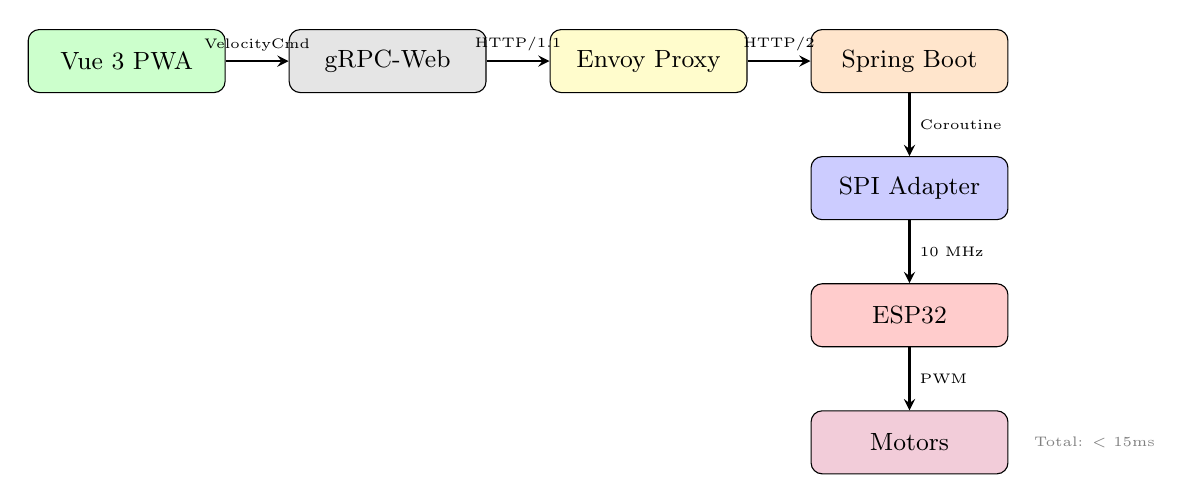
\begin{tikzpicture}[
    node distance=0.8cm,
    box/.style={draw, rectangle, rounded corners, minimum width=2.5cm, minimum height=0.8cm, align=center, font=\small},
    arrow/.style={->, thick, >=stealth}
]
    % PWA
    \node[box, fill=green!20] (pwa) {Vue 3 PWA};

    % gRPC-Web
    \node[box, fill=gray!20, right=of pwa] (grpc) {gRPC-Web};

    % Envoy
    \node[box, fill=yellow!20, right=of grpc] (envoy) {Envoy Proxy};

    % Gateway
    \node[box, fill=orange!20, right=of envoy] (gateway) {Spring Boot};

    % SPI
    \node[box, fill=blue!20, below=of gateway] (spi) {SPI Adapter};

    % ESP32
    \node[box, fill=red!20, below=of spi] (esp32) {ESP32};

    % Motor
    \node[box, fill=purple!20, below=of esp32] (motor) {Motors};

    % Arrows with labels
    \draw[arrow] (pwa) -- node[above, font=\tiny] {VelocityCmd} (grpc);
    \draw[arrow] (grpc) -- node[above, font=\tiny] {HTTP/1.1} (envoy);
    \draw[arrow] (envoy) -- node[above, font=\tiny] {HTTP/2} (gateway);
    \draw[arrow] (gateway) -- node[right, font=\tiny] {Coroutine} (spi);
    \draw[arrow] (spi) -- node[right, font=\tiny] {10 MHz} (esp32);
    \draw[arrow] (esp32) -- node[right, font=\tiny] {PWM} (motor);

    % Latency annotations
    \node[font=\tiny, gray, right=0.2cm of motor] {Total: $<$ 15ms};

\end{tikzpicture}
\caption{Motor Command Data Flow}
\end{figure}

\subsection{SLAM Data Flow}

\begin{figure}[H]
\centering
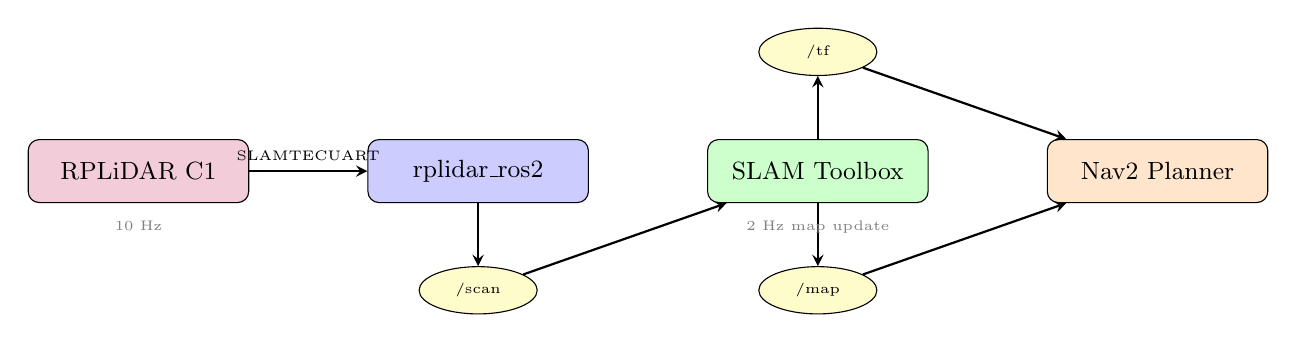
\begin{tikzpicture}[
    node distance=1cm,
    box/.style={draw, rectangle, rounded corners, minimum width=2.8cm, minimum height=0.8cm, align=center, font=\small},
    topic/.style={draw, ellipse, minimum width=1.5cm, minimum height=0.6cm, align=center, font=\tiny, fill=yellow!20},
    arrow/.style={->, thick, >=stealth}
]
    % LiDAR
    \node[box, fill=purple!20] (lidar) {RPLiDAR C1};

    % rplidar_ros2
    \node[box, fill=blue!20, right=1.5cm of lidar] (driver) {rplidar\_ros2};

    % /scan topic
    \node[topic, below=0.8cm of driver] (scan) {/scan};

    % SLAM Toolbox
    \node[box, fill=green!20, right=1.5cm of driver] (slam) {SLAM Toolbox};

    % /map topic
    \node[topic, below=0.8cm of slam] (map) {/map};

    % /tf topic
    \node[topic, above=0.8cm of slam] (tf) {/tf};

    % Nav2 (consumer)
    \node[box, fill=orange!20, right=1.5cm of slam] (nav2) {Nav2 Planner};

    % Arrows
    \draw[arrow] (lidar) -- node[above, font=\tiny] {SLAMTEC\\UART} (driver);
    \draw[arrow] (driver) -- (scan);
    \draw[arrow] (scan) -- (slam);
    \draw[arrow] (slam) -- (map);
    \draw[arrow] (slam) -- (tf);
    \draw[arrow] (map) -- (nav2);
    \draw[arrow] (tf) -- (nav2);

    % Frequency annotations
    \node[font=\tiny, gray, below=0.1cm of lidar] {10 Hz};
    \node[font=\tiny, gray, below=0.1cm of slam] {2 Hz map update};

\end{tikzpicture}
\caption{SLAM Data Flow (ROS 2 Topics)}
\end{figure}

\subsection{Navigation Pipeline}

\begin{figure}[H]
\centering
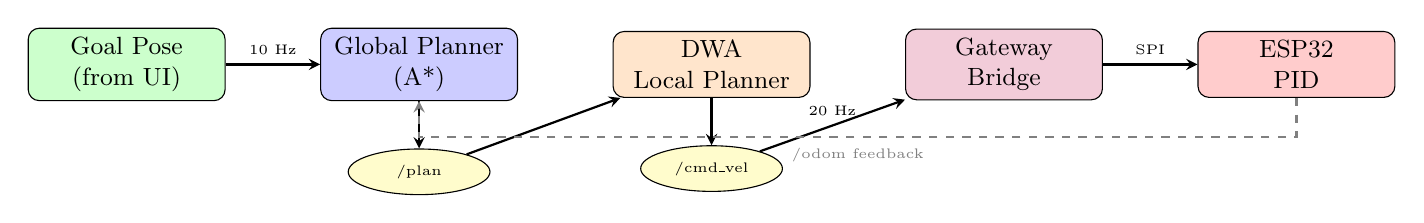
\begin{tikzpicture}[
    node distance=0.6cm,
    box/.style={draw, rectangle, rounded corners, minimum width=2.5cm, minimum height=0.8cm, align=center, font=\small},
    topic/.style={draw, ellipse, minimum width=1.8cm, minimum height=0.5cm, align=center, font=\tiny, fill=yellow!20},
    arrow/.style={->, thick, >=stealth}
]
    % Goal input
    \node[box, fill=green!20] (goal) {Goal Pose\\(from UI)};

    % Global Planner
    \node[box, fill=blue!20, right=1.2cm of goal] (global) {Global Planner\\(A*)};

    % Path topic
    \node[topic, below=0.6cm of global] (path) {/plan};

    % DWA Local Planner
    \node[box, fill=orange!20, right=1.2cm of global] (dwa) {DWA\\Local Planner};

    % cmd_vel topic
    \node[topic, below=0.6cm of dwa] (cmdvel) {/cmd\_vel};

    % Gateway
    \node[box, fill=purple!20, right=1.2cm of dwa] (gateway) {Gateway\\Bridge};

    % ESP32
    \node[box, fill=red!20, right=1.2cm of gateway] (esp) {ESP32\\PID};

    % Arrows
    \draw[arrow] (goal) -- node[above, font=\tiny] {10 Hz} (global);
    \draw[arrow] (global) -- (path);
    \draw[arrow] (path) -- (dwa);
    \draw[arrow] (dwa) -- (cmdvel);
    \draw[arrow] (cmdvel) -- node[above, font=\tiny] {20 Hz} (gateway);
    \draw[arrow] (gateway) -- node[above, font=\tiny] {SPI} (esp);

    % Feedback arrow (odometry)
    \draw[arrow, dashed, gray] (esp.south) -- ++(0,-0.5) -| node[below, font=\tiny, pos=0.25] {/odom feedback} (global.south);

\end{tikzpicture}
\caption{Navigation Pipeline Data Flow}
\end{figure}

\subsection{Telemetry Aggregation Flow}

\begin{figure}[H]
\centering
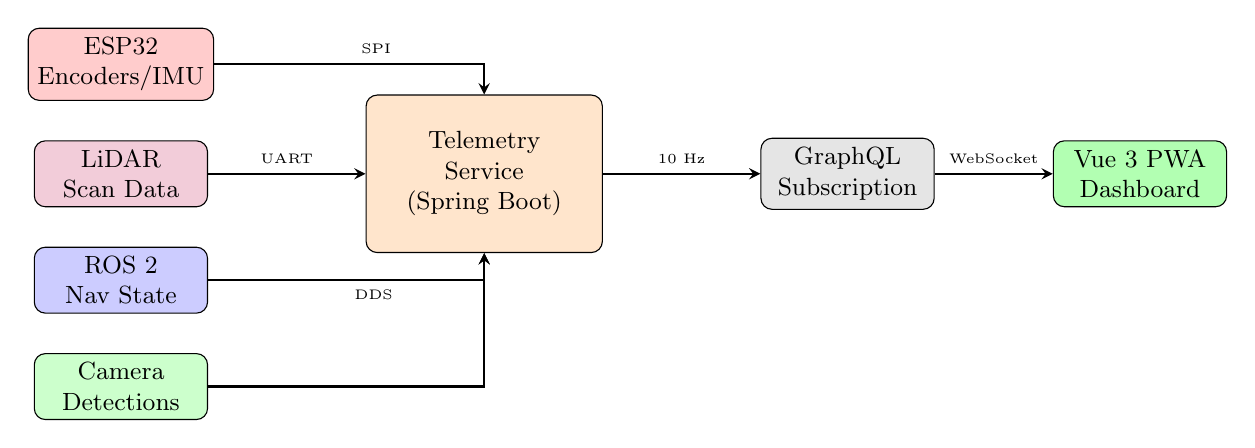
\begin{tikzpicture}[
    node distance=0.8cm,
    box/.style={draw, rectangle, rounded corners, minimum width=2.2cm, minimum height=0.7cm, align=center, font=\small},
    arrow/.style={->, thick, >=stealth}
]
    % Sources (left column)
    \node[box, fill=red!20] (esp) {ESP32\\Encoders/IMU};
    \node[box, fill=purple!20, below=0.5cm of esp] (lidar) {LiDAR\\Scan Data};
    \node[box, fill=blue!20, below=0.5cm of lidar] (ros) {ROS 2\\Nav State};
    \node[box, fill=green!20, below=0.5cm of ros] (camera) {Camera\\Detections};

    % Aggregation service
    \node[box, fill=orange!20, minimum width=3cm, minimum height=2cm, right=2cm of lidar] (agg) {Telemetry\\Service\\(Spring Boot)};

    % Outputs (right column)
    \node[box, fill=gray!20, right=2cm of agg] (graphql) {GraphQL\\Subscription};

    % PWA
    \node[box, fill=green!30, right=1.5cm of graphql] (pwa) {Vue 3 PWA\\Dashboard};

    % Arrows from sources
    \draw[arrow] (esp) -| node[above, font=\tiny, pos=0.3] {SPI} (agg);
    \draw[arrow] (lidar) -- node[above, font=\tiny] {UART} (agg);
    \draw[arrow] (ros) -| node[below, font=\tiny, pos=0.3] {DDS} (agg);
    \draw[arrow] (camera) -| (agg);

    % Output arrows
    \draw[arrow] (agg) -- node[above, font=\tiny] {10 Hz} (graphql);
    \draw[arrow] (graphql) -- node[above, font=\tiny] {WebSocket} (pwa);

\end{tikzpicture}
\caption{Telemetry Aggregation and Publishing}
\end{figure}

% ============================================================================
% SECTION 9: DEPLOYMENT
% ============================================================================
\section{Deployment Configuration}

\subsection{Systemd Service}

\begin{lstlisting}[caption=star-gateway/deployment/star-gateway.service]
[Unit]
Description=STAR Robot Gateway
Documentation=https://github.com/locked-inc/star
After=network-online.target
Wants=network-online.target avahi-daemon.service

[Service]
Type=simple
User=star
Group=star
WorkingDirectory=/opt/star-gateway
ExecStart=/usr/bin/java \
    -Xmx256m \
    -Xms128m \
    -XX:+UseG1GC \
    -XX:MaxGCPauseMillis=50 \
    -Djava.security.egd=file:/dev/./urandom \
    -jar star-gateway.jar

# Restart policy
Restart=always
RestartSec=10
StartLimitInterval=300
StartLimitBurst=5

# Logging
StandardOutput=journal
StandardError=journal
SyslogIdentifier=star-gateway

# Environment
Environment="SPRING_PROFILES_ACTIVE=production"
Environment="JAVA_HOME=/usr/lib/jvm/java-17-openjdk"

# Security hardening
NoNewPrivileges=true
ProtectSystem=strict
ProtectHome=true
PrivateTmp=true
ReadWritePaths=/var/log/star-gateway /var/lib/star-gateway

# Resource limits
MemoryMax=512M
CPUQuota=80%

[Install]
WantedBy=multi-user.target
\end{lstlisting}

\subsection{Avahi mDNS Service}

\begin{lstlisting}[language=XML, caption=star-gateway/deployment/avahi/star-robot.service]
<?xml version="1.0" standalone='no'?>
<!DOCTYPE service-group SYSTEM "avahi-service.dtd">
<service-group>
    <name replace-wildcards="yes">STAR Robot Gateway on %h</name>

    <!-- GraphQL HTTP endpoint -->
    <service>
        <type>_http._tcp</type>
        <port>8080</port>
        <txt-record>path=/graphql</txt-record>
        <txt-record>api=graphql</txt-record>
    </service>

    <!-- GraphQL WebSocket endpoint -->
    <service>
        <type>_ws._tcp</type>
        <port>8080</port>
        <txt-record>path=/graphql-ws</txt-record>
    </service>

    <!-- gRPC endpoint (via Envoy) -->
    <service>
        <type>_grpc._tcp</type>
        <port>8090</port>
        <txt-record>api=grpc-web</txt-record>
    </service>

    <!-- Health check endpoint -->
    <service>
        <type>_http._tcp</type>
        <port>8080</port>
        <txt-record>path=/actuator/health</txt-record>
        <txt-record>api=health</txt-record>
    </service>
</service-group>
\end{lstlisting}

\subsection{Envoy Proxy Configuration}

\begin{lstlisting}[language=yaml, caption=/opt/envoy/envoy.yaml]
admin:
  address:
    socket_address:
      address: 127.0.0.1
      port_value: 9901

static_resources:
  listeners:
    - name: grpc_web_listener
      address:
        socket_address:
          address: 0.0.0.0
          port_value: 8090
      filter_chains:
        - filters:
            - name: envoy.filters.network.http_connection_manager
              typed_config:
                "@type": type.googleapis.com/envoy.extensions.filters.network.http_connection_manager.v3.HttpConnectionManager
                codec_type: AUTO
                stat_prefix: grpc_web

                route_config:
                  name: local_route
                  virtual_hosts:
                    - name: grpc_services
                      domains: ["*"]
                      routes:
                        - match:
                            prefix: "/"
                          route:
                            cluster: grpc_backend
                            timeout: 60s

                      # CORS configuration
                      cors:
                        allow_origin_string_match:
                          - prefix: "*"
                        allow_methods: "GET, POST, OPTIONS"
                        allow_headers: >
                          content-type,
                          x-grpc-web,
                          x-user-agent,
                          grpc-timeout
                        max_age: "1728000"
                        expose_headers: >
                          grpc-status,
                          grpc-message

                http_filters:
                  # gRPC-Web to gRPC translation
                  - name: envoy.filters.http.grpc_web
                    typed_config:
                      "@type": type.googleapis.com/envoy.extensions.filters.http.grpc_web.v3.GrpcWeb

                  # CORS handling
                  - name: envoy.filters.http.cors
                    typed_config:
                      "@type": type.googleapis.com/envoy.extensions.filters.http.cors.v3.Cors

                  # Router
                  - name: envoy.filters.http.router
                    typed_config:
                      "@type": type.googleapis.com/envoy.extensions.filters.http.router.v3.Router

  clusters:
    - name: grpc_backend
      connect_timeout: 0.5s
      type: LOGICAL_DNS
      dns_lookup_family: V4_ONLY
      lb_policy: ROUND_ROBIN
      typed_extension_protocol_options:
        envoy.extensions.upstreams.http.v3.HttpProtocolOptions:
          "@type": type.googleapis.com/envoy.extensions.upstreams.http.v3.HttpProtocolOptions
          explicit_http_config:
            http2_protocol_options: {}
      load_assignment:
        cluster_name: grpc_backend
        endpoints:
          - lb_endpoints:
              - endpoint:
                  address:
                    socket_address:
                      address: 127.0.0.1
                      port_value: 9090
\end{lstlisting}

% ============================================================================
% SECTION 9: IMPLEMENTATION CHECKLIST
% ============================================================================
\section{Implementation Checklist}

\subsection{Phase 1: Infrastructure Setup}

\begin{enumerate}
    \item[$\square$] Create \texttt{star-gateway/} Spring Boot project structure
    \item[$\square$] Create \texttt{proto/} shared protobuf definitions
    \item[$\square$] Set up Gradle build with gRPC + GraphQL plugins
    \item[$\square$] Add Envoy to Buildroot configuration
    \item[$\square$] Configure development environment (IDE, linting, testing)
\end{enumerate}

\subsection{Phase 2: Backend Core}

\begin{enumerate}
    \item[$\square$] Implement \texttt{Esp32SpiAdapter} (Pi4J SPI communication)
    \item[$\square$] Implement \texttt{Esp32TcpAdapter} (TCP fallback)
    \item[$\square$] Implement \texttt{RplidarAdapter} (SLAMTEC protocol via rplidar\_ros2)
    \item[$\square$] Implement domain services:
    \begin{enumerate}
        \item[$\square$] \texttt{MotorControlService}
        \item[$\square$] \texttt{TelemetryService}
        \item[$\square$] \texttt{NavigationService}
        \item[$\square$] \texttt{SensorFusionService}
    \end{enumerate}
    \item[$\square$] Implement GraphQL controllers and schema
    \item[$\square$] Implement gRPC service for motor control
    \item[$\square$] Add Prometheus metrics and health endpoints
    \item[$\square$] Write unit tests for all services
\end{enumerate}

\subsection{Phase 3: Frontend PWA}

\begin{enumerate}
    \item[$\square$] Copy UI-Demo to \texttt{star-ui/}
    \item[$\square$] Add PWA dependencies and Vite PWA plugin
    \item[$\square$] Create Apollo Client with offline persistence
    \item[$\square$] Create gRPC-Web client with proto compilation
    \item[$\square$] Replace \texttt{useMockData} hook with \texttt{useRobotConnection}
    \item[$\square$] Implement IndexedDB storage layer
    \item[$\square$] Create service worker with Workbox
    \item[$\square$] Add offline UI indicators
    \item[$\square$] Test PWA installation and offline mode
\end{enumerate}

\subsection{Phase 4: ESP32 Updates}

\begin{enumerate}
    \item[$\square$] Create \texttt{star\_module\_tcp} library
    \item[$\square$] Implement TCP server with JSON parsing
    \item[$\square$] Add SPI slave command handler (if not present)
    \item[$\square$] Define binary command protocol
    \item[$\square$] Integrate TCP server into \texttt{main.c}
    \item[$\square$] Test SPI + TCP redundancy
\end{enumerate}

\subsection{Phase 5: Deployment}

\begin{enumerate}
    \item[$\square$] Create systemd service file
    \item[$\square$] Create Avahi mDNS service file
    \item[$\square$] Configure Envoy proxy
    \item[$\square$] Update Buildroot to include:
    \begin{enumerate}
        \item[$\square$] OpenJDK 17
        \item[$\square$] Envoy proxy
        \item[$\square$] Gateway JAR
    \end{enumerate}
    \item[$\square$] Create deployment scripts
    \item[$\square$] Integration testing on hardware
\end{enumerate}

\subsection{Phase 6: Documentation}

\begin{enumerate}
    \item[$\square$] Update \texttt{GEMINI.md} with new architecture
    \item[$\square$] Create API documentation (GraphQL schema + gRPC)
    \item[$\square$] Update hardware testing guide
    \item[$\square$] Create troubleshooting guide
    \item[$\square$] Document deployment procedures
\end{enumerate}

% ============================================================================
% SECTION 10: TECHNOLOGY SUMMARY
% ============================================================================
\section{Technology Summary}

\begin{table}[H]
\centering
\small
\begin{tabularx}{\textwidth}{|l|l|X|}
\hline
\textbf{Layer} & \textbf{Technology} & \textbf{Purpose} \\
\hline
\multicolumn{3}{|c|}{\textbf{Frontend (PWA)}} \\
\hline
UI Framework & Vue 3 + TypeScript + Vite 6 & Reactive UI with Composition API \\
PWA & Workbox 7 + Vite PWA & Offline capability, installability \\
GraphQL Client & Vue Apollo 4 + Apollo Client & Data fetching, caching, subscriptions \\
gRPC Client & grpc-web 0.15 & Low-latency motor commands \\
Offline Storage & IndexedDB (idb 8) & Full telemetry history offline \\
Styling & Tailwind CSS 4 & Utility-first responsive design \\
\hline
\multicolumn{3}{|c|}{\textbf{Backend (Gateway)}} \\
\hline
Framework & Spring Boot 3.2 & Production-ready JVM framework \\
Language & Kotlin 1.9 & Modern JVM language with coroutines \\
GraphQL Server & Spring GraphQL & Queries, mutations, subscriptions \\
gRPC Server & grpc-spring-boot-starter 3.1 & Binary RPC for motor control \\
Hardware Access & Pi4J 2.6+ (GpioD) & SPI/GPIO access on RPi5 RP1 chip \\
Metrics & Micrometer + Prometheus & Health monitoring, observability \\
\hline
\multicolumn{3}{|c|}{\textbf{Infrastructure}} \\
\hline
Proxy & Envoy 1.29 & gRPC-Web to gRPC translation \\
Service Discovery & Avahi (mDNS) & Zero-config \texttt{star-robot.local} \\
Process Manager & systemd & Service lifecycle, auto-restart \\
OS & Buildroot 2025.02 LTS & Minimal Linux for RPi5 \\
\hline
\multicolumn{3}{|c|}{\textbf{Firmware (ESP32)}} \\
\hline
Framework & ESP-IDF 5.x & Official Espressif SDK \\
RTOS & FreeRTOS & Real-time task scheduling \\
Communication & SPI + TCP/WiFi & Dual-channel redundancy \\
Architecture & STAR Firmware (DIP) & Modular, testable embedded code \\
\hline
\end{tabularx}
\caption{Complete Technology Stack}
\end{table}

% ============================================================================
% REFERENCES
% ============================================================================
\section{References and Resources}

\subsection{Protocol Documentation}
\begin{itemize}
    \item gRPC Official Documentation: \url{https://grpc.io/docs/}
    \item GraphQL Specification: \url{https://spec.graphql.org/}
    \item gRPC-Web GitHub: \url{https://github.com/grpc/grpc-web}
    \item Spring GraphQL: \url{https://spring.io/projects/spring-graphql}
\end{itemize}

\subsection{Framework Documentation}
\begin{itemize}
    \item Spring Boot 3: \url{https://docs.spring.io/spring-boot/docs/3.2.x/reference/}
    \item Vue Apollo: \url{https://v4.apollo.vuejs.org/}
    \item Workbox: \url{https://developer.chrome.com/docs/workbox/}
    \item Pi4J: \url{https://pi4j.com/documentation/}
\end{itemize}

\subsection{Research References}
\begin{itemize}
    \item Hasura: ``GraphQL vs gRPC'' - \url{https://hasura.io/learn/graphql/intro-graphql/graphql-vs-grpc/}
    \item Stack Overflow Blog: ``When to use gRPC vs GraphQL'' - \url{https://stackoverflow.blog/2022/11/28/when-to-use-grpc-vs-graphql/}
    \item Ambassador Labs: ``Protobuf vs JSON Performance'' - \url{https://www.getambassador.io/blog/protobuf-vs-json}
    \item Postman: ``gRPC vs GraphQL'' - \url{https://blog.postman.com/grpc-vs-graphql/}
\end{itemize}

\subsection{Build Tools}
\begin{itemize}
    \item Vite: \url{https://vitejs.dev/}
    \item Gradle: \url{https://gradle.org/}
    \item PlatformIO: \url{https://platformio.org/}
\end{itemize}

\end{document}
